\documentclass{frontiersSCNS}

\usepackage{url,hyperref,lineno,microtype}
\usepackage[onehalfspacing]{setspace}
\linenumbers

%\usepackage[margin=1in,footskip=0.25in]{geometry}

%\usepackage{helvet}
%\renewcommand{\familydefault}{\sfdefault}

\renewcommand\refname{\vskip -1cm}


%\renewcommand{\rmdefault}{phv} % Arial
%\renewcommand{\sfdefault}{phv} % Arial
\usepackage{setspace}
\usepackage{wrapfig}
\usepackage{amsmath}
\usepackage{amssymb}
\usepackage{graphicx}
\usepackage{mathrsfs}
\usepackage{bm}
\usepackage{wasysym}
\usepackage{placeins}
\usepackage{multirow}
\usepackage[T1]{fontenc}
%\usepackage[super]{natbib}
\usepackage{framed}
\usepackage{caption}
\usepackage{longtable}


\def\keyFont{\fontsize{8}{11}\helveticabold }
\def\firstAuthorLast{Yeakel {et~al.}} %use et al only if is more than 1 author
\def\Authors{
Justin D. Yeakel\,$^{1,2,\dagger,*}$,
Uttam Bhat\,$^{1,3,\dagger}$,
Emma A. Elliott Smith\,$^4$,
and Seth D. Newsome\,$^4$}
% Affiliations should be keyed to the author's name with superscript numbers and be listed as follows: Laboratory, Institute, Department, Organization, City, State abbreviation (USA, Canada, Australia), and Country (without detailed address information such as city zip codes or street names).
% If one of the authors has a change of address, list the new address below the correspondence details using a superscript symbol and use the same symbol to indicate the author in the author list.
\def\Address{$^{1}$Santa Fe Institute, Santa Fe, New Mexico, USA \\
$^{2}$School of Natural Sciences, University of California, Merced, Merced, California, USA \\
$^{3}$Department of Physics, Boston University, Boston, Massachusetts, USA \\
$^{4}$Department of Biological Sciences, University of New Mexico, Albuquerque, New Mexico, USA \\
$^{\dagger}$Contributed equally}
% The Corresponding Author should be marked with an asterisk
% Provide the exact contact address (this time including street name and city zip code) and email of the corresponding author
\def\corrAuthor{Justin D. Yeakel}
\def\corrAddress{Santa Fe Institute, Santa Fe, New Mexico, 87505, USA}
\def\corrEmail{jdyeakel@gmail.com}


\begin{document}
\onecolumn
\firstpage{1}

\title[Exploring the isotopic niche]{Exploring the isotopic niche: isotopic variance, physiological incorporation, and the temporal dynamics of foraging}

\author[\firstAuthorLast ]{\Authors} %This field will be automatically populated
\address{} %This field will be automatically populated
\correspondance{} %This field will be automatically populated

\extraAuth{}% If there are more than 1 corresponding author, comment this line and uncomment the next one.
%\extraAuth{corresponding Author2 \\ Laboratory X2, Institute X2, Department X2, Organization X2, Street X2, City X2 , State XX2 (only USA, Canada and Australia), Zip Code2, X2 Country X2, email2@uni2.edu}


\maketitle


% \begin{document}
%
% \title{Isotopic incorporation and the temporal dynamics of foraging among individuals and within populations}
% \author{JD Yeakel, U Bhatt, SD Newsome}
% \maketitle

\begin{abstract}

%%% Leave the Abstract empty if your article falls under any of the following categories: Editorial Book Review, Commentary, Field Grand Challenge, Opinion or specialty Grand Challenge.
%As a primary goal, the abstract should render the general significance and conceptual advance of the work clearly accessible to a broad readership. References should not be cited in the abstract.
%For full guidelines regarding your manuscript please refer to \href{http://www.frontiersin.org/about/AuthorGuidelines}{Author Guidelines} \\ or \textbf{Table \ref{Tab:01}} for a summary according to article type.
\section{}
Consumer foraging behaviors are dynamic, changing in response to prey availability, seasonality, competition, and even the physiological states of the consumers.
The isotopic composition of a consumer is a product of these factors as well as the isotopic `landscape' of its prey, i.e. the isotopic mixing space.
Stable isotope mixing models are used to back-calculate the most likely proportional contribution of a set of prey to a consumer's diet based on their respective isotopic distributions, however they are disconnected from ecological process.
Here we build a mechanistic framework that links the ecological and physiological processes of an individual consumer to the isotopic distribution that describes its diet, and ultimately to the isotopic composition of its own tissues, defined as its `isotopic niche'.
By coupling these processes, we systematically investigate under what conditions the isotopic niche of a consumer changes as a function of both the geometric properties of its mixing space and foraging strategies that may be static or dynamic over time.
Results of our analytical derivations reveal general insight into the conditions that impact isotopic niche width as a function of consumer specialization on prey, as well as its ability to transition between diets over time.
We show analytically that moderate specialization on isotopically unique prey can serve to maximize a consumer's isotopic niche width, while temporally dynamic diets will tend to result in peak isotopic variance during dietary transitions.
We demonstrate the relevance of our theoretical findings by examining a marine system composed of nine invertebrate species commonly consumed by sea otters.
In general, our analytical framework highlights the complex interplay of mixing space geometry and consumer dietary behavior in driving expansion and contraction of the isotopic niche.
Because this approach is established on ecological mechanism, it is well-suited for enhancing the ecological interpretation, and uncovering the root causes, of observed isotopic data.
%We hope that our process-based framework will expand and enhance the ecological interpretation of isotopic data.


%Here we introduce a statistical framework designed to couple the ecological and environmental processes that determine foraging strategies, the physiological incorporation of isotopes into consumer tissues, and the isotope mixing space of its prey, with the consumer's isotopic distribution, defined as its `isotopic niche'.
%We systematically assess the combined 


\tiny
 \keyFont{ \section{Keywords:} Isotopic niche, Trophic niche, Mixing space, Dietary variation, Specialization, Prey switching} %All article types: you may provide up to 8 keywords; at least 5 are mandatory.
\end{abstract}


\section{Introduction}

Consumer foraging behaviors are dynamic, often resulting in variable diets that change over time and space as a function of environmental conditions, the densities of consumers and available resources, and even the physiological states of individual foragers, to name a few.
Understanding how diets change, and to what extent different conditions promote or inhibit specific changes, is both a challenging theoretical and empirical problem in ecology, but is essential for elucidating the adaptive nature of complex ecological systems.

The comparison of carbon ($\delta^{13}\rm{C}$) and nitrogen ($\delta^{15}\rm{N}$) stable isotope values of a consumer with respect to its potential prey is a commonly utilized approach to quantify diet composition.
The carbon and nitrogen isotopic composition of a consumer represents that of the food it eats, but is offset by predictable amounts, often called trophic discrimination factors, that are mediated by consumer physiology \citep{VanderZanden:2001p2449,Post:2002wn,FoxDobbs:2007kx,Bearhop:2010db}.
%As a consumer incorporates the isotopic values of its resources into its tissues, it becomes a blend of these resources.
The isotopic composition of a consumer thus reflects
1) the proportional contribution of different prey to the consumer's diet \citep{Moore:2008kg,Parnell:2010ub}, and
2) the isotopic composition of its prey, collectively described as the isotopic, or prey, mixing space \citep{Phillips:2001ws,Phillips:2002tu,Newsome:2007tz}.

The isotopic niche of a consumer is a low-dimensional specification of the `Hutchinsonian niche' \citep{Hutchinson:1957tg}, an n-dimensional hypervolume that defines all biotic and abiotic requirements needed for a species to exist.
The isotopic niche is also generally derived from both biotic and abiotic processes, but in contrast to the large and ultimately immeasurable construct of the n-dimensional hypervolume, isotopic niches are defined exactly as a consumer's isotopic variance with a dimension determined by the number of isotope systems employed \citep{Bearhop:2004im,Newsome:2007tz,Newsome:WhhVfocb,delRio:2011p2553,Jackson:2011kd}.
It is the width, or spread of this distribution that correlates to the breadth of the isotopic niche.
Although the isotopic niche can be the result of many ecological and environmental factors that influence the flow of elements through biological systems \citep{Araujo:2007iua}, when it is primarily driven by consumer-resource interactions, the isotopic niche is synonymous with the trophic niche as defined by \citet{Bearhop:2004im}.
Changes in the size of the isotopic niche have been shown to relate to ecosystem fragmentation \citep{Layman:2007ky}, evolutionary diversification \citep{Fedosov:2014hm}, changes in food availability \citep{Lehmann:2015db}, and even individual responses to seasonal environments \citep{delRio:2011p2553}, however a systematic understanding of how different sources of variability influence the isotopic niche is lacking.


Both the consumer's dietary strategy as well as the isotopic mixing space contribute different sources of variability that are reflected in the isotopic composition of the consumer.
For example, a consumer could be an obligate specialist on a single prey, such that its dietary variability is extremely low, in which case the isotopic mean and variability of the consumer's tissues will reflect that of its targeted prey.
In contrast, the consumer could be a generalist, or intermediate specialist on certain prey such that the variability in its diet as well as the isotopic variability of its prey contributes to its own isotopic composition.
Thus, the isotopic composition of a consumer is not only a reflection of what the consumer eats, but is also determined by the mixing space over which it integrates isotope values, and the amount of time over which a particular tissue integrates dietary inputs.
%Thus, the isotopic composition of a consumer contains important information regarding the foraging ecology of the consumer, but is also determined by the mixing space over which it integrates isotope ratios.
%It is this variability that ecologists have coined `the isotopic niche' \citep{Bearhop:2004im,Newsome:2007tz,Newsome:WhhVfocb,Jackson:2011kd,delRio:2011p2553}. %and there has been much focus on the importance of understanding the breadth of this isotopic niche with respect to the  mixing space of a consumer's prey (REFS).


%Individual vs. population
The isotopic niche is generally defined with respect to the isotopic variance of a population \citep{Araujo:2007iua,Araujo:2009p2286,Fink:2012eg}, however population-level variance is itself an artifact of the individual-level distributions from which the population is composed \citep{Bolnick:2007p1253,Araujo:2011gm}.
An important step in understanding how the isotopic niche changes in response to different consumer foraging strategies is to examine how individual-level variation contributions to observed isotopic variability.
Individual-level variability, in particular that variability resulting from temporal changes in diet, has large implications for the population \citep{Kondoh:2003p1625,Kondoh:2006p1622,Schreiber:2011wx}.
For example, populations with greater individual-level variability have been shown to exhibit greater stability \citep{Bolnick:2011gj}, and in certain cases can increase the likelihood of species coexistence \citep{Schreiber:2011wx}.
Changes in individual diet through time is frequently measured via stable isotope analysis of metabolically inert, temporally-integrating tissues such as hair, whiskers, claws, or even growth layers in teeth \citep{Koch:1995vj,Matthews:2004hw,Sponheimer:2006fj,Post:2008ki,Newsome:2009tn,Yeakel:2009hz,Hopkins:2015ip}.


%Bayesian (backwards) vs. simulation (forwards)
Once physiologically-mediated isotopic discrimination between a consumer and its food has been accounted for, the isotopic niche is a direct reflection of the proportional contribution of different prey resources to the consumer's diet.
Isotope mixing models, which originally used a bootstrapping framework \citep{Phillips:2003kq,Phillips:2005p1007} and now employ Bayesian methods \citep{Moore:2008kg,Parnell:2010ub,Hopkins:2012dza,Parnell:2012wv}, are used to reconstruct the probability distribution that describes the contribution of different prey; mixing models can only be solved exactly if the number of potential prey resources are less than or equal to the number of isotope systems used plus one.
These tools are forensic in nature, and can be used to back-calculate consumer diets across a range of isotopically distinct prey with differing stoichiometries \citep{Hopkins:2015ip}, to quantify intra- and inter-population niche variability \citep{Semmens:2009uq}, to reconstruct diets of extinct taxa \citep{Yeakel:2012uc}, and even combined with process-based models that are designed to constrain contribution-to-diet estimates based on known mechanistic relationships between species \citep{Ogle:2014jg}.


%Forward iteration framework... mention Araujo and Fink
A conceptually divergent, yet parallel, strategy is to consider the inter-related effects of ecological interactions and the concomitant integration of stable isotope values, and how these factors combine to result in the isotopic composition of a consumer.
In this way, the consumer's isotopic distribution can be forward-integrated through time based on the mechanistic linkages between its foraging strategy, its ability to find and acquire prey, and the isotopic landscape (mixing space) over which its diet is composed.
This general perspective has been applied to investigate properties of the isotopic niche for cases of fixed (non-varying) diets \citep{Araujo:2007iua,Araujo:2009p2286}, and with respect to experimental systems where consumers are forced to switch between unique prey \citep{Fink:2012eg}.
However, such a process-based framework has not been directly linked to consumer foraging behaviors, prey availability, or other ecological considerations such that the combined impacts of ecologically-mediated dietary variation and mixing space geometry on the isotopic niche can be assessed.



%our measure of specialization different than Araujo... similar to fink???

Here we build a mechanistic framework that links the ecological and physiological processes of an individual consumer to the isotopic distribution that describes its diet, and ultimately to the isotopic composition of its own tissues.
By coupling these processes, we are able to systematically investigate under what conditions the isotopic niche of a consumer changes as a function of both geometric properties of its mixing space, and alternative foraging strategies.
We show that the isotopic variance of a consumer's diet (and by extension the width of its isotopic niche) is expected to be a concave parabolic function with respect to prey specialization, such that it possesses a peak variance, though the appearance of this peak is contingent on mixing space geometry.
We demonstrate the potential importance of these findings by examining a prey mixing space for sea otters (\emph{Enhydra lutris}), which are known to possess high dietary individuality \citep{Estes:2003uc,Tinker:2008tp,Newsome:2009tn,Newsome:2015gy}.

We then extend our framework to explore how a consumer's isotopic niche responds to temporally dynamic diets.
We examine an example of a switch between two probabilistic diets that oscillates between, for example, seasons, and show analytically that the maximum expected isotopic niche width occurs during the transitions between diets.
Determining how different sources of variability emerge from ecological, behavioral, and geometric drivers is important for interpreting the meaning of concepts such as the isotopic niche.
Moreover, integrating these different sources of variation into a statistical process-based framework lends itself particularly well to hypothesis-testing aimed at uncovering the root causes of observed isotopic data.
We hope that our approach is a step towards assessing how the isotopic niche may change due to more complex foraging behaviors and even population dynamics, and we expand on these ideas in the Discussion.



%Determining the most likely proportional contribution of prey that determines a given consumer's diet has thus been the focus of intense interest (REFS).
%
%Of additional interest are the factors that control the consumer's isotopic niche width, which is defined by the isotopic variance of the consumer at either the individual or population level.
%A consumer's isotopic niche width, by definition, is a function of the isotopic values of its potential prey (the prey mixing space), as well as its dietary predilections.
%For a given mixing space, a consumer with a large isotopic niche width may be incorporating many isotopically distinct prey into its diet, while a consumer with a small isotopic niche width may be specializing on a single resource.


%Difference between the isotopic diet view vs. other diet views

%Backward integrating vs. Forward integrating

%EXPLORE VARIANCE ~ what controls the isotopic niche?

%Prey-switching dynamic
%Micro time frame
%Macro time frame




\section{Methods \& Analysis}
We begin by establishing a forward-integration approach for modeling the incorporation of stable isotopes from multiple resources into a consumer's tissues.
This new methodology provides an analytical link between the mechanistic drivers of foraging and the distribution of stable isotope values describing a consumer's tissues over time.
%This framework aims to provide a flexible platform for introducing additional ecological complexities, such as time-dependent foraging behaviors and dietary specialization both among and within individuals.
Using this framework, we aim to
1) examine how certain dietary behaviors, such as prey specialization and different modes of dietary variation, impact the isotopic variance of consumer tissues, and
2) show how these methods can be expanded to include foraging behaviors that themselves are temporally dynamic, changing over seasons or years.
Accordingly, our general goal is to reveal how both ecological and geometric factors can influence the expansion and contraction of isotopic variability, thus aiding ecological interpretation of the `isotopic niche'.


\subsection*{Deriving the within-individual isotopic niche width}
%The dynamics of diet ~ heuristic description of the process
There are many ways to statistically summarize the integration of prey by a consumer species, however in order to establish a mechanistic link between foraging and the consumer's isotopic composition, we follow the proceeding heuristic foraging mechanic.
We assume that a consumer encounters and consumes resources in proportion to the encounter rate of each prey; prey that are encountered more frequently are assumed to be consumed more frequently.
An alternative approach could incorporate preferences \citep{Chesson:1983bt} or even state-dependence \citep{Mangel:1988uaa,Clark:2000tra,Mangel:2014kz}, and we will briefly address these considerations in the Discussion.
As prey are encountered and consumed, the prey's isotope values are incorporated into the consumer's tissues weighted by the prey-specific proportional contribution to diet.
The resulting distribution that describes the dietary input of multiple prey (each with  isotope values that are independently and Normally distributed) is a mixed Normal distribution with weights determined by the prey's proportional contribution to diet.
This proportional contribution is itself a random variable drawn from a Dirichlet density (a multivariate Beta distribution) that serves as a probabilistic description of the consumer's dietary input \citep{Ainsworth:2010uo}.
The following section details our probabilistic determination of the consumer's isotopic composition.
We focus our attention on the variability of the isotopic distribution describing the consumer's diet, which scales directly with the consumer's own isotopic distribution, which is itself equivalent to the isotopic niche \citep{Bearhop:2004im,Newsome:2007tz}.
Here and henceforth, we assume that the isotope ratios under consideration follow dietary pathways such that the isotopic niche is synonymous with the trophic niche \citep{Bearhop:2004im}.
% a statistic of certain interest to ecologists using stable isotopes as a tool to understand diet.
%, as well as an analysis of the properties of the final consumer isotopic distribution.


%Derivation of the Dirichlet controlling diet
%If we  that the proportional contribution of prey to a consumer's diet scales to the rate at which it encounters its prey.
%, such that we must first describe how the Dirichlet distribution describing consumer diet at a given point in time changes as a function of prey densities.
A consumer encounters each prey at a frequency determined by a Poisson process with parameter $\psi_i$, which determines the number of encounters $M_i=m_i$ between time 0 and time $t$, with the frequency distribution

\begin{equation}
f_{M_i} (m_i|\psi_i) = {\rm e}^{-\psi_i t}\frac{(\psi_i t)^m_i}{m_i!}.
\end{equation}

\noindent Here and henceforth, we use the general function $f(\cdot)$ to denote different frequency distributions, as well as uppercase notation to describe stochastic variables, and lowercase notation to describe specific values of stochastic variables.
If we assume that encounter rates are variable, such that some prey are more patchily distributed than others, we can treat $\Psi_i = \psi_i$ as a random variable with a Gamma density

\begin{equation}
f_{\Psi_i} (\psi_i | c, a_i) = \frac{c^{a_i}}{\Gamma (a_i)}{\rm e}^{-c \psi_i}\psi_i^{a_i - 1}.
\end{equation}

\noindent Here, $a_i$ is the dispersion parameter, which is proportional to the encounter rate, and $c$ scales with the time between encounters \citep{Mangel:2006wa,Ainsworth:2010uo,Yeakel:2013hi}.
If we integrate across all possible values of $\psi_i$, we obtain the Negative Binomial density with mean encounter rate $a_i/c$ and coefficient of variation $1/\sqrt{a_i}$ \citep{Hilborn:1997ds}.
Following the derivation described by \citet{Ainsworth:2010uo}, if we define the proportional contribution of prey to a consumer's diet to scale with the encounter rate, such that

\begin{equation}
\label{eqp}
  p_i = \frac{\psi_i}{\sum_{j=1}^n \psi_j},
\end{equation}

\noindent then the random variable $P_i = p_i$ where $P_i \in {\bm P}$ and $p_i \in {\bm p}$, and $\sum_i p_i = 1$, and note that we allow boldface type to denote vectors of variables.
From Eq. \ref{eqp}, it follows that the vector describing the proportional contributions to diet $\bm P$ follows a Dirichlet distribution \citep{Johnson:1960gu} with density

\begin{equation}
  f_{\bm P}(p_1,...,p_n|a_1,...,a_n) = \frac{\Gamma(\sum_{i=1}^n a_i)}{\sum_{i=1}^n\Gamma(a_i)}\prod_{i=1}^n p_i^{a_i - 1},
\end{equation}

\noindent where $\Gamma(\cdot)$ is the gamma function \citep[cf.][]{Mangel:2006wa}.
%We note that bold-face fonts denote vectors of variables.
As such, the expected proportional contribution of a prey $i$ to the consumer's diet has the expectation ${\rm E}\{P_i\}=a_i/a_0$ where $a_0 = \sum_i a_i$, and variance

\begin{equation}
  \label{eqDirVar}
  {\rm V}\{P_i\} = \frac{a_i(a_0 - a_i)}{a_0^2(a_0 + 1)}.
\end{equation}

\noindent In this paper we consider the case where resources are plentiful and feeding is regular, and we draw a single prey $i$ with probability $p_i$ for inclusion to the consumer's diet.
%Accordingly, we assume each time interval represents a single foraging bout, where we draw a single prey $i$ with probability $p_i$ for inclusion to the consumer's diet.

Describing the dietary behavior of a consumer as a Dirichlet distribution provides a flexible and powerful framework to investigate how different foraging strategies influence a consumer's isotopic niche.
For example, a pure generalist consumer would have a Dirichlet distribution with parameters $a_i = 1$ for all prey $i=1,...,n$, such that the marginal distribution for $P_i$ is close to uniform with expectation ${\rm E}\{P_i\} = 1/n$.
Because we have assumed that the proportional contribution of a prey to the consumer's diet scales with the prey's encounter rate, this would be analogous to a system where a consumer is equally likely to encounter the same number of any prey.
In contrast, an obligate specialist would have a Dirichlet density that is spiked for a given prey $k$, such that the single parameter $a_k \gg 1$, while $a_{i \neq k} = 1$.
The use of a Dirichlet distribution is also at the heart of Bayesian isotope mixing models \citep{Moore:2008kg,Parnell:2010ub,Hopkins:2012dza,Parnell:2012wv}, which assume a Dirichlet prior and enable the input of alternative dietary information to inform isotopic data.



%Describing Z
If the stable isotope ratios for each of the potential prey follow independent Normal distributions, and the dietary behavior of the consumer has a Dirichlet density, the resultant density that describes the isotopic distribution of a consumer's diet $f_Z(Z=z)$ is a mixed Normal distribution, with weights given by $\bm p$ drawn from the Dirichlet.
Given that the isotopic means and variances for prey $i$ are denoted by $\mu_i$ and $\sigma^2_i$, respectively, this density can be written as

%\begin{equation}
%  \label{eqfZ}
%f_Z(z|{\bm p},{\bm \mu},{\bm \sigma}) = \sum_{i=1}^n p_i\frac{1}{\sqrt{2 \pi \sigma_i^2}}{\rm e}^{-\frac{(z-\mu_i)^2}{2\sigma_i^2}},
%\end{equation}

\begin{equation}
  \label{eqfZ}
f_Z(z|{\bm a},{\bm \mu},{\bm \sigma}) = \left(\sum_{i=1}^n p_i\frac{1}{\sqrt{2 \pi \sigma_i^2}}{\rm e}^{-\frac{(z-\mu_i)^2}{2\sigma_i^2}}\right)f_{\bm P}(\bm p | \bm a),
\end{equation}


\noindent with the expectation

\begin{equation}
\label{eqEZ}
  {\rm E}\{Z\} = \sum_{i=1}^n \frac{a_i}{a_0} \mu_i,
\end{equation}

\noindent Accordingly, the isotopic mean of the consumer's diet is a weighted average of the isotopic means of its potential prey, where weights are determined by the outcome of the Dirichlet random variable.
%where weights are determined by the mean proportional contribution of prey to the consumer's diet.

Of more interest to us here is the variance of $Z$, which will allow us to analytically determine the isotopic niche width of the consumer as a function of its dietary behavior and the mixing space of its prey.
We find that

\begin{equation}
\label{eqVarZ}
  {\rm V}\{Z\} = \sum_{i=1}^n \frac{a_i}{a_0}\left(\sigma_i^2 + \mu_i^2\right) - \frac{a_i^2\mu_i^2}{a_0^2}-\sum_{i \neq j}\frac{a_i a_j \mu_i \mu_j}{a_0^2}.
\end{equation}

\noindent Although the form of Eq. \ref{eqVarZ} is not intuitive, we emphasize that - over different dietary behaviors that shape the Dirichlet distribution and for different isotopic mixing spaces - it is this equation that governs the expansion or contraction of the consumer's isotopic niche width, and therefore of chief ecological interest.

The isotopic variance of the consumer's diet ${\rm V}\{Z\}$ can be simplified by considering a specific set of dietary behaviors.
Here we examine how ${\rm V}\{Z\}$ is influenced by generalist vs. specialist consumer diets, as well as the role of general mixing space geometries, in determining consumer isotopic niche width.
It is important to note that specialism, as discussed here defines the degree to which a consumer's diet is dependent on a single prey resource, ranging from $s=1/n$ (obligate generalization) to $s=1$ (obligate specialization).
It is thus conceptually different than `individual specialization' defined as the proportional variance of an individual relative to that of its population \citep[Within-Individual Component / Total Niche Width, or WIC/TNW;][]{J:1979wc}, and often the variable of interest in other studies examining properties of the isotopic niche \citep{Araujo:2007iua,Araujo:2009p2286,Araujo:2011gm,Layman:2011cm}.

If a generalist consumer alters its diet to include more of a certain prey $k$ relative to the others, the Dirichlet distribution that defines its dietary behavior goes from $a_i=1$ for all $i=1,...,n$ to $a_{i \neq k}=1$ for $i=1,...,n$, with $a_k>1$.
As specialization increases, the Dirichlet parameter corresponding to the targeted prey $k$ increases to a value much higher than one (pure specialization is obtained only at the limit $a_k \to \infty$).
Thus, we can assume that $a_i=1$ for all $i \neq k$, and $a_k = (n-1)s_k/(1-s_k)$, where $s_k$ denotes specialization on prey $k$. %ranging from $1/n$ (generalization) to $1$ (specialization).
We can thus substitute $a_0 = (n-1)/(1-s_k)$ and $p_i = a_i/a_0 = (1-s_k)/(n-1)$ for all $i \neq k$, and $a_k/a_0 = s_k$.
We can then rewrite Eq. \ref{eqVarZ} as

\begin{equation}
\label{eqVarZs}
{\rm V}\{Z\} = \frac{1-s_k}{n-1}\sum_{i \neq k}^n \left(\sigma_i^2 + \mu_i^2\right) + s_k(\sigma_k^2 + \mu_k^2) - \left(\frac{1-s_k}{n-1}\sum_{i \neq k}^n \mu_i + s_k\mu_k \right)^2,
\end{equation}

\noindent and note that, independent of the prey mixing space (a function of $\mu_i$ and $\sigma_i^2$ for prey $i=1,...,n$), the isotopic variance of the consumer's diet will always be a concave parabolic function over $s_k$.
With respect to the size of the consumer's isotopic niche width, this means that there can be a peak variance for a value of $s_k$ intermediate to pure generalization ($s_k=1/n$) and pure specialization ($s_k=1$).

The peak variance $\hat s_k$, which describes the maximum isotopic variance of the consumer, may or may not fall between $s_k=1/n$ and $s=1$, and is only of ecological interest if it does.
The peak variance can be solved analytically by setting the derivative of Eq. \ref{eqVarZs} with respect to $s_k$ equal to zero, and solving for $s_k$, which results in

\begin{equation}
	\hat s_k = \frac{A(1-n)+B (n-1)^2+2 C (C-D n+D)}{2 (C-D n+D)^2},
\end{equation}

\noindent where $A = \sum_{i \neq k}^n \left(\sigma_i^2 + \mu_i^2\right)$, $B = \left(\sigma_k^2 + \mu_k^2\right)$, $C = \sum_{i \neq k}^n \mu_i$, and $D = \mu_k$.

Determination of the peak variance allows us to predict where the consumer's isotopic niche is expected to be maximized as a function of specialization on different prey.
Although here we have focused on the special case where a consumer targets a single prey, one can rewrite the equation for the consumer's isotopic niche width with respect to increasing specialization on any number or combination of prey in the mixing space.
For example, in the case where a consumer specializes on two prey (e.g. two species of crab), one would rewrite Eq. \ref{eqVarZ} in terms of both $s_k$ (specialization on prey $k$) and $s_l$ (specialization on prey $l$), resulting in a concave parabolic plane in dimensions $s_k$ and $s_l$.
Determining the maximum variance would then entail taking the derivative of Eq. \ref{eqVarZ} with respect to both $s_k$ and $s_l$.
In dimensions higher than 2, the process would be the same, with the goal of finding the maximum variance over a hyperplane with a number of dimensions determined by the number of prey on which the consumer is preferentially targeting.
Because specializing on multiple prey does not introduce anything conceptually unique, we consider only the case of a single-prey specialist.



\subsection*{The Dynamics of Isotopic Incorporation}
We have established a framework for analytically calculating the distribution of isotope values that characterizes a consumer's diet, composed of multiple, isotopically distinct prey.
The dietary behavior of the consumer is a function of a single Dirichlet distribution, which is assumed not to change over time, although we will relax this assumption in the next section.
Over long timescales the dietary distribution of the consumer is static, with a fixed mean and variance.
Over short timescales, the consumer's diet varies as Eq. \ref{eqDirVar}, while its final isotopic distribution has a variability emerging from the combined effects of the Dirichlet and the mixed Normal distribution describing the prey mixing space (Eq. \ref{eqVarZ}).

%Not sure, but this might be more appropriate in the discussion
As the consumer acquires and consumes its prey, the isotopic composition of its diet is incorporated into its tissues.
The timescale of physiological incorporation is based on the turnover rate of consumer tissues, which on the fast end can occur within days to weeks (e.g. blood plasma), and on the slow end occur over years (e.g. bone) \citep{Tieszen:1983ij}, and can be estimated via controlled feeding studies \citep{Kurle:2009ch,Bearhop:2010db,Kim:2012kc}. %and occasionally in the wild (REFS?).
Although the physiological details are not well understood, isotopic incorporation can be modeled using either single- or multi-compartmental approaches \citep{Cerling:2006kv,delRio:2008bs}.
In a single compartment framework, isotope ratios are ingested with food, and directly incorporated into consumer tissues at a tissue-specific rate.
In multiple compartment frameworks, it is assumed that incorporation occurs over multiple body pools, the turnover of each potentially occurring at different rates.
Though an assumption of multi-compartmental incorporation can provide better statistical fit with experimental data \citep{Cerling:2006kv,Kurle:2009ch,Carleton:2008cq}, the physiological processes that drive incorporation of isotope ratios from one compartment to the other are not well understood \citep{delRio:2008bs}, and for many tissues single-compartment models fit as well or better than multi-compartment models \citep{Kurle:2009ch}.

In this next section, we assume that the ingested isotope ratios are incorporated into consumer body tissues directly, moderated by the rate of incorporation $\lambda$, which is treated as a free parameter.
Here we consider only a single compartment model, such that isotope ratios are directly shuttled to consumer tissues at rate $\lambda$; we note, however, that functions for multi-compartment models could be used instead, though we do not expect large qualitative differences in results \citep[cf. Fig. 1 in][]{delRio:2008bs}.
For simplicity, we assume that time is scaled such that a single time step corresponds to a single foraging bout.
Moreover, we assume that the consumer is incorporating prey of smaller size than itself, such that $ 0 < \lambda < 1$.
Thus, we aim to determine the isotopic composition of the consumer $X_c$ as a function of its diet, the isotopic mixing space, and $\lambda$.
We note 1) that the isotopic composition of the consumer could represent its carbon ($\delta^{13}{\rm C}$) or nitrogen ($\delta^{15}{\rm N}$) isotope value, and our proceeding derivations work equivalently for both, and 2) that all trophic discrimination factors are assumed to have been accounted for, such that $X_c$ directly reflects the consumer's diet.
% The carbon and nitrogen isotope composition of a consumer's tissues are a product of its diet.
% If this diet incorporates multiple prey in different quantities, as is the case for most consumers, the resulting consumer isotopic distribution must take into account:
% \emph{i}) the initial isotopic signature of the consumer's tissues at a point in time $X_c(t)$ (we will assume for simplicity that the isotopic value in question is the ratio of heavy to light carbon isotope relative to a known standard $\delta^{13}{\rm C}$, though are methods are equivalent for any isotope that is integrated through diet),
% \emph{ii}) the isotopic values of $n$ resources, which we assume are Gaussian distributed with expectation $\mu_i$ and variance $\sigma_i^2$,
% %$\sum_{i=1}^n p_i \mu_i$ (where $p_i$ is the proportional contribution of resource $i$ and $\mu_i$ is the mean isotopic value of resource $i$),
% \emph{iii}) the rate at which each prey species is ingested by the consumer, summarized by its proportional contribution $p_i$,
% and
% \emph{iv}) the incorporation rate of a consumer's diet into its tissue $\lambda$.
In a completely deterministic framework, the isotopic composition of the consumer over time $t$ can be written as an ordinary differential equation, where

\begin{equation}
\label{eqODE}
\frac{\rm d}{\rm dt} X_c(t) = \lambda \sum_{i=1}^N p_i \mu_i - \lambda X_c(t).
\end{equation}

%\noindent where $t$ is time, and $p_i$ and $\mu_i$ are the proportional contribution of prey $i$ to the diet of the consumer, and the mean isotope value of prey $i$, respectively.

However, we must also take into account the stochastic effects described in the previous section, including the variation associated with the consumer's diet and the isotopic variation associated with each prey.
We account for these stochastic effects by describing changes in the consumer's isotopic distribution with the stochastic differential equation

\begin{equation}
\label{eqSDE}
{\rm d}X_c(t) = \lambda\left({\rm E}\{Z\}{\rm dt} + \sqrt{{\rm V}\{Z\}}{\rm dW}\right) - \lambda X_c(t){\rm dt}.
\end{equation}

\noindent where ${\rm dW}$ is the increment of Brownian motion.
This stochastic differential equation describes an Ornstein-Uhlenbeck process, which is a stochastic process that has a steady state variance around the mean \citep{Mangel:2006wa}.
Because the time interval ${\rm dt}$ is infinitesimal at the continuous limit, the consumer's isotopic distribution will have a Normal distribution.
In this case, if the initial isotopic values of the consumer at time $t=0$ is $X_c(0)$, the expectation and variability of $X_c$ at time $t$ are

\begin{align}
  \begin{split}
    \label{eqEVar}
{\rm E}\{X_c(t)\} &= {\rm E}\{Z\} + (X_c(0) - {\rm E}\{Z\}){\rm e}^{-\lambda t},\\
{\rm V}\{X_c(t)\} &= \frac{\lambda {\rm V}\{Z\}}{2}\left(1 - {\rm e}^{-2\lambda t}\right).
\end{split}
\end{align}

\noindent where ${\rm E}\{Z\}$ and ${\rm V}\{Z\}$ are as defined in Eqns. \ref{eqEZ} and \ref{eqVarZ}.
One can observe that as $t$ increases, the exponential part of ${\rm E}\{X_c(t)\}$ and ${\rm V}\{X_c(t)\}$ go to zero, such that ${\rm E}\{X_c(t)\} \to {\rm E}\{Z\}$, and ${\rm V}\{X_c(t)\} \to \lambda{\rm V}\{Z\}/2$.
In other words, the expectation of the consumer's isotopic distribution will equilibrate to that of its diet, while its variance will always be less than the variance of its diet by a factor of $\lambda/2$.
Variance decreases as the rate of incorporation decreases due to the consumer averaging its isotopic value over more prey (because the tissue is turning over more slowly), and this serves to average out fluctuations in the consumer's diet.
% This decrease in variance is due to the fact that the consumer-diet mix has a biased weight towards its own body tissues, such that $\lambda < 1(2)$.
%if \lamabda = 2, then it will look like what it eats... weird... worth going into at all?




% This is in accordance with known exponentially-decaying isotopic values of consumers shown in controlled-diet experiments (REFS).

%By uniting both dietary and isotopic variability into the single random variable $Z$, the above framework provides a means towards predicting the isotopic composition of a consumer over time, given a dietary strategy (described by the Dirichlet distribution) and the isotopic distribution of the potential resources (the isotopic mixing space).
%Permitting the consumer's dietary strategy to vary provides a direct means of incorporating behavioral variability in estimates of a consumer's isotopic composition.





%\subsection*{Temporal dietary dynamics}
Our static model is defined by a consumer's diet that varies instantaneously over a given parameterization of $f_Z(z)$.
This is relevant for organisms that have a consistently varying diet over time, however most organisms have diets that undergo large, qualitative changes over longer periods time.
In such cases, the Dirichlet distribution that characterizes diet during one small temporal interval will be different than the Dirichlet distribution characterizing diet during another interval far apart in time.
Such a shift might be due to seasonal, ontogenetic, or demographic changes in the consumer or its prey base over the course of months, or years, depending on the timescale of interest.
In the following section, we will relax the assumption that diet is characterized by a single Dirichlet distribution, thus generalizing our formulation of consumer isotopic dynamics as a function of time.

The random variable of interest is now $Z(t)$, which is the trajectory defining the isotopic distribution of the consumer's diet over time.
Solving for $X(t)$, we find

\begin{align}
  \label{eqEVarZt}
{\rm E}\{X(t)\} = X(0){\rm e}^{-\lambda t} + \lambda{\rm e}^{-\lambda t} \int_{s=0}^t {\rm e}^{\lambda s} {\rm E}\{Z(s)\}{\rm d}s, \nonumber \\
{\rm V}\{X(t)\} = \lambda^2 {\rm e}^{-2\lambda t} \int_{s=0}^t {\rm e}^{2\lambda s} {\rm V}\{Z(s)\} {\rm d}s.
\end{align}

\noindent By defining the temporal dynamics of diet $Z(t)$ and the incorporation rate $\lambda$, we can thus analytically determine the isotopic mean and variance of the consumer's tissues.


%\noindent and this is conceptually analogous to the formulation of consumer isotopic variance as derived by \citet{Fink:2012eg}.

% Incorporating different classes of prey-switching dynamics permits an understanding of how the isotopic composition of a consumer reflects changes in its behavior over time as a function of the incorporation rate $\lambda$.
% To gain an intuitive understanding of how ecological dynamics are portrayed by consumer isotope values, we consider two types of prey-switching behavior: {\it i}) an instantaneous shift from one dietary strategy to another (such as those used in feeding experiments), and {\it ii}) a sinusoidally varying dietary strategy.




\section{Results}

% As a consumer samples from multiple prey with stable isotopes values following independent Normal distributions, its tissues become a mixture of these distributions.
% The weights that control the contributions of each prey to the consumer mix are determined by the dietary behavior of the consumer, which we have shown follows a Dirichlet distribution.
% The use of the Dirichlet distribution in this context follows , and is also used as a prior in Bayesian isotope mixing models.
% We note that Bayesian mixing models are essentially models that explore the opposite question that we are investigating: they are used to estimate the dietary behavior of the consumer (the posterior probability distribution for the proportional contribution vector $\bm p$) given the isotopic distributions of both consumer and prey, whereas we are investigating factors that impact the isotopic distribution of the consumer as a function of different prey mixing spaces and consumer dietary behaviors.


We have provided an analytical solution for the mean and variance of the consumer's isotope distribution as a function of its diet and the prey mixing space.
By formulating these solutions in terms of consumer generalization and specialization (Eq. \ref{eqVarZs}), we make three observations:
1) the variance of the isotopic distribution of the consumer's diet, ${\rm V}\{Z\}$, which scales to its isotopic niche width, is concave parabolic (Fig. \ref{figvar}); 
2) whether and to what extent ${\rm V}\{Z\}$ demonstrates measurable nonlinearity depends in part on the geometry of the mixing space;
3) the peak variance over the generalization-specialization continuum is the consumer's maximum isotopic niche width.
This point may or may not exist at a value intermediate to an obligate generalist and obligate specialist.


The nonlinear nature of the consumer's isotopic niche width as a function of its specialization on certain prey (or combinations of prey) is driven almost entirely by the geometry of the prey mixing space.
One can gain some intuitive understanding of this nonlinearity by considering the following example, illustrated in Fig. \ref{figvar}.
In a three-prey system, where all prey have equal isotopic means and variances, a consumer that ranges from generalization on all three prey to specialization on a single prey will likewise have isotopically equivalent diets.
As the mean isotope value of the targeted prey is moved away from the others, such that its offset from the mixing space centroid \citep[the center of the mixing space;][]{Layman:2007vi,Newsome:WhhVfocb} is increased, the variance function displays increasing nonlinearity.
%This can be understood by considering two prey with the same mean value, and the targeted prey with a very different mean value.
For a skewed mixing space, where one prey source has a very different isotope composition than the rest \citep[e.g. a mixing space consisting of terrestrial foods vs. a marine subsidy;][]{Newsome:2004p992}, if the consumer incorporates isotopes from all three sources in equal proportions (a generalist), it will have relatively higher isotopic variance than if its prey exhibited a less skewed mixing space geometry.
The skewness of the mixing space increases with the offset of the targeted prey from the mixing space centroid as shown in Fig. \ref{figvar}.
As the consumer integrates this isotopically unique prey in greater proportions, the heterogeneity of incorporated isotope values will increase, serving to increase the consumer's isotopic variability.
The isotopic variability will then decline as the consumer begins specializing on the atypical prey, and if it is consuming this prey exclusively, the isotopic variability of its diet will reflect the isotopic variability of its prey exactly.
The concave parabolic nature of the isotopic variability of the consumer's diet can thus be explained by heterogeneous incorporation of isotope ratios over an skewed, or asymmetric, mixing space.


%3: Peak variance location
Understanding what dietary strategy or mixing space geometry can maximize the isotopic niche width of the consumer's diet will serve to help ecologists determine what mechanisms - ecological or statistical - may be driving patterns in isotope data, or whether these mechanisms can be decoupled at all.
Our analytical solution for peak variance over dietary specialization on prey $k$, $\hat s_k$, reveals that maximum isotopic niche width can, but doesn't always, fall in $s_k \in [1/n,1]$, with bounds denoting exclusive prey generalization or specialization, respectively.
If the peak lies outside of this region, changes in isotopic variance as specialization on a targeted prey is increased will appear monotonic or even linear.

Although the specific nature of $\hat s_k$ will depend strongly on mixing space geometry, we can elucidate certain key attributes that will determine the general nature of where this value falls.
For mixing space geometries where the targeted prey has higher than average variance, $\hat s_k$ will tend to lie towards prey specialization ($s_k>0.5$), however the offset of the mean value of the targeted prey from the mixing space centroid will quickly push $\hat s_k$ to $s_k \to 0.5$ (Fig. \ref{figspecvar}A,B).
In contrast, if the targeted prey has lower than average variance, $\hat s_k$ will tend to lie towards prey generalization ($s_k < 0.5$; Fig. \ref{figspecvar}B,C).
As before, if the offset of the targeted prey's mean value increases, $\hat s_k \to 0.5$.
In both cases, if the mean value for the targeted prey is close to the mixing space centroid, the maximum isotopic variance for the consumer could lie in any region.




\subsection*{Temporally variable diets}
%Incorporation results
The equilibrial solution to our stochastic differential equation (Eq. \ref{eqEVar}) reveals that the isotopic variability of the consumer scales to diet as a factor of $\lambda/2$.
As the incorporation rate decreases, such that the turnover time is longer, the isotopic variability of the consumer declines.
This is due to the consumer averaging its tissues over a greater number of foraging bouts.
Moreover, we observe that as the consumer transitions from some initial isotopic state $X_c(0)$ to diet, the variance of the consumer's isotopic values equilibrate twice as fast as the mean value.

%Dynamic diet results
If the consumer's diet is itself variable over time, we do not expect its isotopic composition to equilibrate as it would in a controlled feeding study (Eq. \ref{eqEVarZt}).
For example, the consumer might adopt one diet during the wet season, and another during the dry season, such that it oscillates between the two throughout the year.
We consider a composite diet with an isotopic distribution $\mathbb{Z}(t) \sim f_{\mathbb{Z}}(t)$ that dynamically oscillates between two subdiets, which we will refer to as `seasonal diets' with frequency $\omega$.
We note that $1/\omega$ in this context corresponds to the `dietary correlation time' of \citet{Fink:2012eg}.
Seasonal diets have random variables $Z_1$ and $Z_2$, each distributed according to Eq. \ref{eqfZ}, though they have different underlying Dirichlet distributions -- encoding which prey the consumer targets during each season with frequency distributions $f_{\bm P_1}$ and $f_{\bm P_2}$ -- while the isotopic distributions of prey are assumed to be constant over time.
We can thus describe the composite diet as a mix of the seasonal diets characterized by weights that oscillate over time, and this determines the contribution of each seasonal dietary strategy to the whole.
We define $\mathcal{U}(t)$ to be the proportional contribution of $Z_1$ to the composite diet $\mathbb{Z}(t)$ over time, such that it can vary between zero (no incorporation of $Z_1$) to unity (complete reliance on $Z_1$).
The frequency distribution for the composite diet is thus

% \begin{equation}
%   f_{\mathbb{Z}(t)} = \left(\mathcal{U}(t) \sum_{i=1}^n p_{1,i}{\rm Gaus}_i( z | \mu_i,\sigma_i) + (1-\mathcal{U}(t)) \sum_{i=1}^n p_{2,i}{\rm Gaus}_i( z | \mu_i,\sigma_i)\right)f_{\bm P_1}f_{\bm P_2}
% \end{equation}

\begin{equation}
  f_{\mathbb{Z}(t)} = \mathcal{U}(t) f_{Z_1} + (1-\mathcal{U}(t)) f_{Z_2}. %f_{\bm P_1}f_{\bm P_2}.
\end{equation}

% \noindent where $\rm Gauss_i( z | \mu_i,\sigma_i)$ is the Gaussian distribution describing the isotope values for prey $i$, while $f_{\bm P_1}$ and $f_{\bm P_2}$ are the Dirichlet distributions for subdiets 1 and 2, respectively.
% \noindent where $f_{Z_1}$ and $f_{Z_2}$ are independent mixed distributions as defined in Eq. \ref{eqfZ} for diets 1 and 2, while $f_{\bm P_1}$ and $f_{\bm P_2}$ are the Dirichlet distributions for subdiets 1 and 2, respectively.

If we do not specify the type of oscillation that drives changes in diet over time, the expectation and variance for the isotopic distribution of the composite diet over time are thus

\begin{align}
  \label{eqZtgen}
  \begin{split}
    {\rm E}\{\mathbb{Z}(t)\} &= \mathcal{U}(t){\rm E}\{Z_1\} + (1-\mathcal{U}(t)){\rm E}\{Z_2\}, \\
    {\rm V}\{\mathbb{Z}(t)\} &= \mathcal{U}(t){\rm V}\{Z_1\} + (1-\mathcal{U}(t)){\rm V}\{Z_2\} + \mathcal{U}(t)(1-\mathcal{U}(t))\left({\rm E}\{Z_1\} - {\rm E}\{Z_2\}\right)^2,
  \end{split}
\end{align}

\noindent where the isotopic mean of the composite diet is averaged over both seasonal diets, weighted by the proportional inclusion of each.
In the wet/dry season example, the consumer could either shift gradually from its wet season diet to its dry season diet if $\mathcal{U}(t)$ is smooth, or shift abruptly if $\mathcal{U}(t)$ is discontinuous.
%An example of the latter scenario would be a grizzly bear consumer system, where its diet shift abruptly with the arrival of salmon during spawning season (REF).


Dietary transitions between seasons tend to be gradual, even if the start/end of a given season is abrupt \citep{Thompson:1995co,CodronSAJWR2007}.
To understand how a temporally oscillating diet affects the isotopic variance of the composite diet, we consider the smooth oscillation $\mathcal{U}(t) = 1/2 + 1/2\sin(\omega t)$, such that the proportional contribution of $Z_1$ oscillates with frequency $\omega$ (Fig. \ref{figvarZt}A).
Substituting $\mathcal{U}(t)$ into Eq. \ref{eqZtgen} provides the solution to a sinusoidally varying diet, with expectation and variance

\begin{align}
  \begin{split}
  \label{eqZtsin}
  	{\rm E}\{\mathbb{Z}(t)\} &= \frac{{\rm E}\{Z_1\} + {\rm E}\{Z_2\}}{2} + \frac{{\rm E}\{Z_1\} - {\rm E}\{Z_2\}}{2}\sin(\omega t), \\
    {\rm V}\{\mathbb{Z}(t)\} &= \overbrace{\frac{{\rm V}\{Z_1\} + {\rm V}\{Z_2\}}{2} + \frac{1}{2} \left(\frac{{\rm E}\{Z_1\} - {\rm E}\{Z_2\}}{2}\right)^2}^{\alpha_{\rm V}} \\
    &+ \overbrace{\frac{{\rm V}\{Z_1\} - {\rm V}\{Z_2\}}{2}}^{\beta_{\rm V}}\sin(\omega t) + \overbrace{\frac{1}{2}\left(\frac{{\rm E}\{Z_1\} - {\rm E}\{Z_2\}}{2}\right)^2}^{\gamma_{\rm V}}\sin\left(2\omega t + \frac{\pi}{2}\right).
  \end{split}
\end{align}

\noindent where we have combined the non-oscillating components of the variance into three parameters $\alpha_{\rm V}$, $\beta_{\rm V}$, and $\gamma_{\rm V}$ for notational efficiency.

We gain three key insights from the solution for the expectation and variance of the composite diet.
1) As would be expected, the central tendency of the composite diet is the average of the mean values for each subdiet, while the amplitude of oscillations is driven entirely by the difference in the mean values of each subdiet;
2) the time-averaged variance (denoted by $\langle \cdot \rangle_t$) is simply $\langle {\rm V}\{\mathbb{Z}(t)\} \rangle_t = \alpha_{\rm V}$, which is only impacted by the average variance between the seasonal diets and the difference in the mean isotope values between the seasonal diets (Fig. \ref{figvarcont});
3) the oscillating component shows that the composite dietary variance has a modified frequency, as well as an offset, meaning that the maximal variance of the consumer's composite diet generally occurs during the transition from one diet to the other (Fig. \ref{figvarZt}B).
Together, these results reveal that if the consumer's diet is varying continuously over time between two seasonal diets, both the averaged variance, as well as the difference in the mean isotope values of the seasonal diets -- directly reflecting the heterogeneity of prey mixing space geometry -- will serve to increase the time-averaged variance of the consumer's diet, and by extension the isotopic variance of the consumer itself.

Less intuitively, we observe that the consumer's peak variance, or niche width, as measured by the variance of its composite diet, occurs not during the exclusive adoption of its subdiets, but during the transition between the two, and this peak variance is driven exclusively by the difference in means between seasonal diets.
As the seasonal diets become more heterogeneous in isotopic space, the greater the consumer's peak variance during the transition, and this occurs because it is sampling between two dietary strategies that are isotopically distinct.
We can directly observe this by considering a transition between two diets with  a) different means and the same variances, and b) the same means and different variances.
In the former case, the peak variance of the composite diet occurs during the transition (Fig \ref{figvarZt}B); in the latter case, because the diets have the same mean isotope value, the peak occurs not during the transition, but when the consumer adopts the diet with the greater variance, which in our example would occur at the height of the season (Fig \ref{figvarZt}C).

%Consumer diet X_c(t)
The isotopic composition of a consumer $X_c(t)$ during a single dietary shift is governed by a single timescale of physiological origin: the rate of incorporation $\lambda$ (Eq. \ref{eqEVar}).
However, a seasonally shifting diet that is driven by oscillating foraging strategies introduces an additional ecological timescale that will affect $X_c(t)$, determined by the frequency of diet switching $\omega$ (Fig. \ref{figxcsin}A).
Depending on the turnover rate of the tissue of interest and how often the consumer shifts its diet, the ratio of these timescales $\omega/\lambda$ will impact how the isotopic mean and variance of the consumer changes over time.
For the case of a sinusoidally varying diet, we can solve for $X_c(t)$ directly, such that

\begin{align}
  \label{eqXsin}
  \begin{split}
    {\rm V}\{X_c(t \gg 0)\} = &\alpha_{\rm V}\frac{\lambda}{2} + \beta_{\rm V}\frac{\lambda^2}{\sqrt{(2\lambda)^2 + \omega^2}}\sin\left(\omega t -\theta_1\right) \\
    &+ \gamma_{\rm V}\frac{\lambda^2}{2\sqrt{\lambda^2 + \omega^2}}\sin\left(2\omega t + \theta_2\right).
  \end{split}
\end{align}

\noindent where the offsets $\theta_1$ and $\theta_2$ are $ \tan^{-1}(\omega/2\lambda)$ and $ \tan^{-1}(\lambda/\omega)$, respectively.
As in the case of a single diet $Z$, the time-averaged variance is scaled by the incorporation rate as $\alpha_{\rm V}\lambda/2$.
Moreover, we observe that the consumer's isotopic composition lags behind changes in diet, such that an isotopic shift in the consumer's tissues is observed after the actual foraging shift.
This lag involves both $\theta_1$ and $\theta_2$, however these offsets play different roles in contributing to the lag for different mixing space geometries.
When the isotopic means of the seasonal diets are similar, the lag is mostly due to $\theta_1$; when the means are different and the variances are similar, the lag is mostly due to $\theta_2$; when both the isotopic means and variances of the seasonal diets are different, both contribute significantly to the lag.
%We can quantify the timing of this shift from Eq. \ref{eqXsin}, and observe that it is XXXX.


As shown in Fig. \ref{figxcsin}, we observe that
%Increasing $\omega/\lambda$, such that the timescale of ecological switching relative to that of isotopic incorporation decreases,
1) the lag between the transition and the peak variance of the consumer increases with decreasing $\lambda$ (i.e. increasing timescale of incorporation), and
2) the amplitude of the variance of $X_c(t)$ decreases with increasing $\omega$ (i.e. decreasing timescale of ecological switching).
The first result is not surprising, as it mirrors the role of $\lambda$ in the static diet example. %when diet did not change over long periods of time.
The second result is less intuitive: in words, as the consumer shifts its diet more frequently, there is still a peak variance during dietary transitions, though with diminishing amplitude, and this would make it more difficult to measure (Fig \ref{figxcsin}B).
This is due to the consumer slowly integrating isotopes into its tissues from both diets, thus averaging across diet-switching events, thus dampening fluctuations.
Accordingly, the decrease in the amplitude of isotopic variance of the consumer's tissue is an averaging effect, where the timescale of incorporation is much larger than the timescale of dietary switching.
%Accordingly, we observe that as a consumer adopts a more frequently shifting diet, changes in its variance will become more damped and difficult to measure, while as the rate of incorporation decreases, the lag between shifts in diet and the isotopic value of the consumer will increase.





\section{Discussion}

%General - Emphasize the importance of peak variance (this should echo the discussion)
%The use of stable isotope ratios in ecology has increased exponentially in the last twenty years \citep{Boecklen:2011fu}.
%Recent development of tools designed to increase the utility of using stable isotope ratios to infer diet have focused almost exclusively on Bayesian mixing models \citep[for a review, see][]{Parnell:2012wv}.
%Bayesian isotope mixing models are extremely useful for backwards-estimating the probability distribution the described the proportional contribution of each species to the consumer's diet, where both the isotopic composition of the consumer and potential prey are known.
%However, there are many cases where these tools cannot be used, and this may be due to
%1) incomplete knowledge of the mixing space (REFS),
%2) an isotopically confounded mixing space (REFS), or
%3) under-sampling of the consumer and/or its potential prey.

We have established a forward-integration approach towards understanding how the isotopic distribution of an individual consumer evolves due to ecological, physiological, and geometric factors.
Our framework introduces mechanistic links between the ecological foraging dynamics of a consumer, the physiological constraints that dictate incorporation, and the more abstract effects of mixing space geometry.
%This approach  replace the utility of isotope mixing models \citep[for a review, see][]{Parnell:2012wv}, but instead offers an opposing framework by which the underlying drivers that result in the isotopic composition of a consumer can be understood.
%Where isotope mixing models are aimed on answering the question: `what was the most likely dietary behavior of the consumer given the isotope values of itself and its prey', we explore how different ecological scenarios and mixing space geometries can alter the isotopic composition of a consumer individual.
We focus our efforts on building an analytical framework to understand how the isotopic variance of an individual -- its isotopic niche width -- changes as a function of different foraging strategies that are both probabilistic and dynamic over time.
%In constructing an analytical approach towards understanding isotopic variance at the individual consumer level, we have found uncovered certain relationships between  that will be important to consider when one is interpreting the isotopic variation of consumers over different timescales.
We consider two foraging scenarios:
1) {\it static strategy}: probabilistic consumption of multiple prey, the proportions of which are on average constant over time, and
2) {\it dynamic strategy}: probabilistic consumption of multiple prey whose relative contribution to consumer's diet varies over time.
The former example is most relevant for consumers inhabiting environments where resource availability is stable (reliable), whereas the latter is more appropriate for consumers that prey switch between two qualitatively different subdiets.

Our primary findings concern whether and to what extent the peak isotopic variance of the consumer, or maximum isotopic niche width, is realized under different, but definable, conditions with respect to static and dynamic foraging scenarios.
When the consumer exhibits a static foraging strategy, the isotopic variance of its diet is tied directly to its prey specialization and the skewness of the isotopic mixing space.
We show that as the mixing space becomes more skewed, there is an increasing likelihood that the peak variance will occur at intermediate specialization (where a single prey accounts for ca. 50\% of the consumer's diet; Figs. \ref{figvar},\ref{figspecvar}).
When the consumer exhibits a dynamic, yet smoothly varying foraging strategy, we show that the peak variance occurs during the transition from one diet to another, and is offset by a lag that is a function of both its incorporation rate and the timescale over which it shifts between diets (Fig. \ref{figvarZt}).
Below we show that these findings are relevant beyond theory by examining an empirical sea otter mixing space, and discuss areas where additional realism can be incorporated to gain further ecological insight into the isotopic niche.


%Static
\subsection*{The isotopic niche: generalization vs. specialization}

%Revisit the results of specialization


%Otter example
To demonstrate the empirical relevance of the nonlinear nature of ${\rm V}\{Z\}$, we examine a prey-rich marine system near San Simeon and Monterey Bay, California, composed of nine invertebrate species commonly consumed by sea otters \citep{Tinker:2008tp}.
In this system, all potential prey resources have unique isotopic means and variances (Fig. \ref{figsomix}), including multiple species of sea urchins and crab, clams, abalone, mussels, and snails.
We can investigate how alternatively targeting each prey species alters the isotopic variance of a sea otter's diet across different degrees of specialization by modifying the underlying Dirichlet distribution (i.e. by increasing $a_k$ for each species individually, while holding $a_{i \neq k} = 1$; Fig. \ref{figottervar}A).
We determined the existence of strong nonlinearity in the isotopic variance of diet for 44\% of prey species (Fig. \ref{figottervar}B). %, due to both the magnitudes of each prey's means and variances relative to that of the remaining prey 
For targeted prey exhibiting nonlinear variance (including mussels, snails, purple sea urchins, and kelp crabs), the maximum isotopic variance was found in the region $s \leq 0.5$.

The message that we take from the sea otter example is relatively straightforward: for a given prey mixing space, a consumer's dietary variability -- where the consumer's tissues scale in proportion to its diet by a factor of $\lambda/2$ -- will be a function of both mixing space geometry, as well as its dietary strategy, and these effects can be confounding.
Despite this, we are able to establish certain predictions for the consumer's isotopic niche width as a function of diet: as the consumer incorporates moderate amounts of isotopically unique prey into its diet, its variance will be expected to increase.
Knowledge of the interplay between mixing space geometry and a consumer's dietary strategy, and its consequent effect on the isotopic variance of diet, is particularly important for characterizing consumers based exclusively on isotopic variance.
For example, without knowledge of these relationships, a highly variable consumer might be interpreted as a dietary generalist, whereas it might be able to achieve a similarly high or higher variance by moderately focusing its foraging activities on a single prey species with an isotopic distribution far from the mixing space centroid.



%Temporal dynamics discussion
\subsection*{The isotopic niche over time}

We gain additional insight into the factors influencing consumer isotopic variability by considering dynamic diets, where the consumer oscillates between different foraging strategies over time.
We considered a simple sinusoidal oscillation for $\mathcal{U}(t)$, the proportional contribution of diet 1 to the composite diet over time $\mathbb{Z}(t)$.
The subdiets from which the composite diet is composed can be thought of as `seasonal diets'.
Our analytical results showed that the peak variance of the composite diet occurred during the transition between seasonal diets.
Importantly, this is not due to any particular mixing space geometry, but a general result that will always occur, as long as the diets are isotopically distinct (each with a unique mean and variance), and the transition is smooth such that a consumer gradually shifts between different diets, as opposed to an abrupt, discontinuous diet switch.

Although the peak variance of $\mathbb{Z}(t)$ is entirely due to ecological diet shifts rather than mixing space geometry, the latter does play a role in determining the mean value (time average) of ${\rm V}\{\mathbb{Z}(t)\}$.
The effect of mixing space geometry on the time-averaged variance of the composite diet is determined by $\alpha_{\rm V}$, which is a function of
1) the average variance of the subdiets from which $\mathbb{Z}$ is composed, and
2) the mean difference between the two subdiets (see Eq. \ref{eqXsin}).
As either of these factors increase, the average variance of the composite diet increases, setting the baseline from which the peak dietary variance fluctuates (Fig. \ref{figvarcont}).
We also observed that as the frequency of dietary transitions increased relative to the rate at which the consumer integrates dietary isotopes into its tissues, the consumer's isotopic variance exhibited lower amplitude as it fluctuated between the different variances of its diet (Fig. \ref{figxcsin}).
This occurs because the greater transition frequencies serve to average variance of the two diets within its tissues.
\citet{Fink:2012eg} found a similar dynamic when they derived an analytical solution for the variance of a consumer population transitioning between two prey.
%As the frequency of dietary transitions increased, the variance of the consumer population became small, effectively because the individual consumer diets increased the averaging effects of the two prey; as the frequency decreased, the variance of the population approached that of the prey.


%Continuous vs. discontinuous switch
An interesting observation that we gain from exploring a sinusoidal dietary shift is that the variance peak observed during dietary transitions is dependent on the smoothness of the transition.
In fact, it is the transition mid-point, at $\mathcal{U}(t) = 0.5$, where the composite diet is pulled equally from each seasonal diet, and this serves to maximize the isotopic heterogeneity of the mixture (the consumer).
Thus, when foraging strategies are dynamic, it is the point of maximum isotopic heterogeneity that results in peak isotopic variance of the diet.
This is analogous to the cause of peak dietary variance in the static example, where specialization on prey resources with greater isotopic offsets from the mixing space centroid maximizes isotopic heterogeneity, resulting in a variance peak.

An extreme alternative to a smooth dietary transition would be one that is discontinuous, as depicted by a step-function, or square wave (Fig. \ref{figsawtooth}A).
Such an instantaneous dietary shift is not ecologically unrealistic; e.g. both brown bears and gray wolves abruptly shift their diet to salmon during salmon runs \citep{Hilderbrand:1999kq,Darimont:2002ex,Levi:2012ir}, as do predators on other prey populations exhibiting localized boom-bust dynamics such as locusts, krill, jellyfish, and sardines \citep{Dawson:2008hj,Atkinson:2014jm}.
Because there is no point during a sharp, discontinuous transition that serves to mix subdiets, the variance of the composite diet does not peak in response.
Instead, both the expectation and the variance of the composite diet incorporates this step function behavior, transitioning to reflect the shifts between different diets.
Because the isotope ratios associated with diet are incorporated gradually into the consumer's tissues, both the mean and the variance of the consumer will adopt a sawtooth-like dynamic (Fig. \ref{figsawtooth}A,B), where they begin to asymptote to the expectation and variance of the subdiets, but are reverted abruptly at the dietary switch.
We note that, as in the static example, the isotopic variance of the consumer approaches the variance of its diet twice as fast as its expectation (cf. Eq. \ref{eqEVar}).

\subsection*{Population dynamics and state-dependent foraging}
%Introducing preferences and/or state dependence thought
We presented a simple dynamic-switching framework, where a consumer oscillates between two different diets over time to explore its effect on its isotopic niche.
In reality, a consumer's dietary strategy might be shifting constantly over time, in response to a constantly changing environment.
One potentially important extension of our framework could incorporate a population dynamic underlying the availability of potential resources (and by extension the consumer's diet) in a continuous, more complex, and ecologically justified manner.
Our original formulation of the Dirichlet distribution that describes the consumer's diet was established on the relationship between the random variables describing the proportional contribution of prey to diet ($P_i = p_i$) and its encounter rate ($\Psi_i = \psi_i$), where $p_i = \psi_i/\sum_j \psi_j$, and this was assumed to have a static distribution over time.
However, if the prey are fluctuating in accordance to an underlying population dynamic (for example, determined by a system of differential equations), the encounter rate of each prey would itself be a function of time.
By relating the expectation and/or variance of $\Psi_i$ to the density of prey, the parameterization of the Dirichlet can be directly coupled to changes in population densities, thus mechanistically incorporating population dynamics into predictions of a consumer's isotopic composition.
%This would enable one to build a hypothesis-testing framework based on the effect of cert
%, allow us to build predictions of a consumer's isotopic composition as a function of these dynamics.


Furthermore, the relationship between $p_i$ and $\psi_i$ explicitly assumes passive foraging between the consumer and its potential prey, and this holds for our original static (single diet) example, our shifting diet example, and would hold for the example above where the Dirichlet changes in response to an underlying population dynamic.
Although this is not a bad starting point, and may be a perfectly reasonable assumption for a filter feeder that consumes resources indiscriminately, it is not a reliable assumption for most organisms that may rank prey based on intrinsic traits (e.g., energetic yield, handling/processing time).
Instead, a more complex relationship between $p_i$ and the attributes of the consumer's prey, and perhaps attributes of the consumer itself, could be used to determine the parameterization of the Dirichlet distribution defining the consumer's diet over time.


For example, our framework implicitly assumes that there is a steady state influx of prey biomass to match the metabolic expenses of the consumer.
In other words, prey are chosen in accordance to the Dirichlet distribution, but it is assumed that each foraging bout contributes equally to the consumer's diet, and that the consumer always finds a meal.
In reality, the success of a given foraging bout is not certain, and there is some risk of not finding any prey at all \citep{Creel:2008p838}; in such a case, the consumer would resort to metabolizing its own tissues \citep{Doucett:1999bz,VanderZanden:2001p2449}.
Such a dynamic would directly impact the rate of incorporation by altering the proportional contribution of newly consumed isotopes to the turnover of the consumer's body tissues.
Moreover, the foraging decisions that a consumer makes are often a function of its energetic state \citep{Barnett:2007er,Yeakel:2013hi}, which changes as it successfully or unsuccessfully finds and acquires its prey \citep{Mangel:1986um}.
Such state-dependent foraging may be difficult to treat analytically, but could be explored numerically, and this approach would be useful for hypothesis testing, particularly when one is interested in comparing the effects of different foraging strategies on the statistical properties of the consumer's isotopic composition.

%Linking our approach to population dynamics
%U(t) is the solution to a population-dynamic equation



%%Why the individual is important...
%Individuals vs. populations
%KEY: High variance of individuals will lead to high variance at the population level
\subsection*{From individuals to populations}
Finally, the framework that we have presented has focused entirely on the individual, in particular on how the isotopic variance of an individual consumer changes in response to different ecological and physiological factors as well as aspects of the isotope mixing space it utilizes.
Most ecological applications using stable isotope analysis operate at the level of the population, although there is a rich literature of efforts that use stable isotope analysis to understand sources of isotopic variation at the level of the individual \citep{Koch:1995vj,Matthews:2004hw,Sponheimer:2006fj,Post:2008ki,Newsome:2009tn,Yeakel:2009hz,Newsome:WhhVfocb,Hopkins:2015ip}.

Understanding how variance percolates from prey to the individual consumer is a necessary first step for understanding sources of isotopic variation at population level.
Such considerations quickly become complex, as there are scenarios when the isotopic variance of an individual is or is not closely coupled to the variance of the population.
For example, if individuals within a population have similar means and - for simplicity - equal variances, then the variance of the population will scale linearly with the variance of the individuals (Fig. \ref{figindpopvar}A,B).
This relationship highlights an important message: when individuality is low, the variance of the population is entirely explained by the variance of the individuals; this means that the results that we have presented for a consumer individual are expected to scale directly to that of the population. 
However, if the individuals within a population have very different means and relatively small variances, then there will not be a significant relationship between population-level and individual-level variation (Fig. \ref{figindpopvar}C,D).
%Accordingly, we expect that our determination of peak variances due to both mixing space and ecological interactions at the individual level to also be true at the population level, as long as the individuals within the population are isotopically similar.

We can imagine different individual-population relationships occurring within a 2-D state-space defined by individuality on one axis and specialization on the other.
At the extremes, a population could consist of
1) obligate specialists with low individuality where all individuals specialize on the same resource,
2) obligate specialists with high individuality where all individuals specialize on different resources, and
3) obligate generalists with low individuality where all individuals are generalists; an obligate generalist with high individuality cannot exist in this context. %such that the individuality-specialization state-space is a triangle.
These potential end-members are discussed at length in \citet{Bearhop:2004im} and \citet{Fink:2012eg}.
As we have seen in the above analyses, the variation of individuals is driven by a complex interplay between mixing space geometry, consumer foraging behaviors, and physiological incorporation.
How these different population-level end-members might shape both individual and population-level isotopic distributions is an important question, though the answers will likely harbor additional complexities.
For example, isotopically similar individuals with low variances imply that all individuals are consuming similar things, in similar quantities, such that individuality is low, though our results show that low isotopic variance need not indicate specialization or generalization \emph{per se} (cf. Figs \ref{figvar},\ref{figottervar}).
Accounting for individual variation in dietary proclivities over time is bound to complicate interpretation further.
%See \citet{Bearhop:2004im} and \citet{Fink:2012eg} for an overview and quantitative analysis of these issues, respectively.

%Of greater potential interest, and relevant to the framework that we have presented, is the scenario in which individuals have different diets that are themselves shifting in time.
%Our approach could be used to hypothesis-test potential ecological/population/behavioral mechanisms that might contribute to the observed isotopic distributions at both the individual and population level, and this would be particularly powerful if one had access to tissues that accumulate over time such as hair, whiskers, claws, growth layers in teeth, or even multiple tissue types which integrate over different temporal scales (i.e., bone and liver).




%Indeed, one can extrapolate what we have learned about variance at an individual level to that of the population.
%For example, the variance of a population -- which is itself defined as a mixture of individuals, each with their own isotopic distribution -- is directly related to the variance of individuals within the population (fig. \ref{figindpopvar}).
%Thus, our determination of variance peaks at the individual level would certainly be `echoed' at the population level, though there are added complications, such as the heterogeneity of individual mean isotope values, that we do not explore here.
%

\subsection*{Conclusions}

%Final statement
There are many sources of variation that contribute to a consumer's isotopic composition.
These sources include the geometry of the prey mixing space, the foraging behaviors of the consumers, as well as temporal changes in the environment that might alter the ability of the consumer to find, acquire, and consume its prey.
%Of recent interest among ecologists using stable isotopes to quantify trophic interactions is the width of a consumer's isotopic niche. %which we have interpreted to be its isotopic variance.
Along with physiological incorporation of isotopes into consumer tissues, these factors serve to drive the temporal evolution of the isotopic distribution, or isotopic niche, of the consumer.
By coupling the isotopic variance of this distribution to mechanistic relationships between the consumer and its diet, as well as the isotopic mixing space of the system, we have presented a systematic exploration of the factors that cause the isotopic niche to both expand and contract.
Incorporating the effects of population dynamics and/or more complex foraging strategies will enable hypothesis testing of different ecological mechanisms to generate the isotopic distributions that are observed in nature.
We hope that such a forward-integrating approach, alongside the use of tools such as mixing models to back-calculate dietary composition, will serve to expand and enhance the ecological interpretation of isotopic data.

\section*{Disclosure/Conflict-of-Interest Statement}
%Frontiers follows the recommendations by the International Committee of Medical Journal Editors (http://www.icmje.org/ethical_4conflicts.html) which require that all financial, commercial or other relationships that might be perceived by the academic community as representing a potential conflict of interest must be disclosed. If no such relationship exists, authors will be asked to declare that the research was conducted in the absence of any commercial or financial relationships that could be construed as a potential conflict of interest. When disclosing the potential conflict of interest, the authors need to address the following points:
%•	Did you or your institution at any time receive payment or services from a third party for any aspect of the submitted work?
%•	Please declare financial relationships with entities that could be perceived to influence, or that give the appearance of potentially influencing, what you wrote in the submitted work.
%•	Please declare patents and copyrights, whether pending, issued, licensed and/or receiving royalties relevant to the work.
%•	Please state other relationships or activities that readers could perceive to have influenced, or that give the appearance of potentially influencing, what you wrote in the submitted work.

The authors declare that the research was conducted in the absence of any commercial or financial relationships that could be construed as a potential conflict of interest.

\section*{Author Contributions}
%When determining authorship the following criteria should be observed:
%•	Substantial contributions to the conception or design of the work; or the acquisition, analysis, or interpretation of data for the work; AND
%•	Drafting the work or revising it critically for important intellectual content; AND
%•	Final approval of the version to be published ; AND
%•	Agreement to be accountable for all aspects of the work in ensuring that questions related to the accuracy or integrity of any part of the work are appropriately investigated and resolved.
%Contributors who meet fewer than all 4 of the above criteria for authorship should not be listed as authors, but they should be acknowledged. (http://www.icmje.org/roles_a.html)
JDY, UB, EAES, and SDN conceived the idea. 
JDY and UB designed the statistical framework and conducted the analyses. 
EAES and SDN contributed empirical data. 
All authors contributed equally to drafting and writing the manuscript. 
%The statement about the authors and contributors can be up to several sentences long, describing the tasks of individual authors referred to by their initials and should be included at the end of the manuscript before the References section.


\section*{Acknowledgments}
We thank C.E. Chow, A. Jakle, Z.D. Sharp, F.A. Smith, and the Center for Stable Isotopes Brown Bag Symposium at the University of New Mexico for helpful comments and discussions that greatly increased the quality of this manuscript.


\textit{Funding\textcolon} J.D. Yeakel was supported by the Omidyar Postdoctoral Fellowship at the Santa Fe Institute.

%\section*{Supplemental Data}
%Supplementary Material should be uploaded separately on submission, if there are Supplementary Figures, please include the caption in the same file as the figure. LaTeX Supplementary Material templates can be found in the Frontiers LaTeX folder

\newpage
\section*{References}

%\bibliographystyle{frontiersinSCNS_ENG_HUMS} % for Science, 
%\bibliography{aa_dyniso}


\begin{thebibliography}{51}
\providecommand{\natexlab}[1]{#1}
\expandafter\ifx\csname urlstyle\endcsname\relax
  \providecommand{\doi}[1]{doi:\discretionary{}{}{}#1}\else
  \providecommand{\doi}{doi:\discretionary{}{}{}\begingroup
  \urlstyle{rm}\Url}\fi
\providecommand{\selectlanguage}[1]{\relax}
\providecommand{\bibAnnoteFile}[1]{%
  \IfFileExists{#1}{\begin{quotation}\noindent\textsc{Key:} #1\\
  \textsc{Annotation:}\ \input{#1}\end{quotation}}{}}
\providecommand{\bibAnnote}[2]{%
  \begin{quotation}\noindent\textsc{Key:} #1\\
  \textsc{Annotation:}\ #2\end{quotation}}

\bibitem[{Ainsworth et~al.(2010)Ainsworth, Kaplan, Levin, and
  Mangel}]{Ainsworth:2010uo}
Ainsworth, C.~H., Kaplan, I.~C., Levin, P.~S., and Mangel, M. (2010).
\newblock {A statistical approach for estimating fish diet compositions from
  multiple data sources: Gulf of California case study}.
\newblock \emph{Ecol. Appl.} 20, 2188--2202
\bibAnnoteFile{Ainsworth:2010uo}

\bibitem[{Ara{\'u}jo et~al.(2011)Ara{\'u}jo, Bolnick, and
  Layman}]{Araujo:2011gm}
Ara{\'u}jo, M.~S., Bolnick, D.~I., and Layman, C.~A. (2011).
\newblock {The ecological causes of individual specialisation}.
\newblock \emph{Ecol. Lett.} 14, 948--958
\bibAnnoteFile{Araujo:2011gm}

\bibitem[{Ara{\'u}jo et~al.(2007)Ara{\'u}jo, Bolnick, Machado, Giaretta, and
  dos Reis}]{Araujo:2007iua}
Ara{\'u}jo, M.~S., Bolnick, D.~I., Machado, G., Giaretta, A.~A., and dos Reis,
  S.~F. (2007).
\newblock {Using $\delta$$^{13}$C stable isotopes to quantify individual-level
  diet variation}.
\newblock \emph{Oecologia} 152, 643--654
\bibAnnoteFile{Araujo:2007iua}

\bibitem[{Ara{\'u}jo et~al.(2009)Ara{\'u}jo, Bolnick, Martinelli, Giaretta, and
  dos Reis}]{Araujo:2009p2286}
Ara{\'u}jo, M.~S., Bolnick, D.~I., Martinelli, L.~A., Giaretta, A.~A., and dos
  Reis, S.~F. (2009).
\newblock {Individual-level diet variation in four species of Brazilian frogs}.
\newblock \emph{J. Anim. Ecol.} 78, 848--856
\bibAnnoteFile{Araujo:2009p2286}

\bibitem[{Bearhop et~al.(2004)Bearhop, Adams, Waldron, Fuller, and
  Macleod}]{Bearhop:2004im}
Bearhop, S., Adams, C.~E., Waldron, S., Fuller, R.~A., and Macleod, H. (2004).
\newblock {Determining trophic niche width:~a novel approach using stable
  isotope analysis}.
\newblock \emph{J. Anim. Ecol.} 73, 1007--1012
\bibAnnoteFile{Bearhop:2004im}

\bibitem[{Bolnick et~al.(2007)Bolnick, Svanback, Ara{\'u}jo, and
  Persson}]{Bolnick:2007p1253}
Bolnick, D., Svanback, R., Ara{\'u}jo, M., and Persson, L. (2007).
\newblock {Comparative support for the niche variation hypothesis that more
  generalized populations also are more heterogeneous}.
\newblock \emph{Proc. Natl. Acad. Sci. USA} 104, 10075
\bibAnnoteFile{Bolnick:2007p1253}

\bibitem[{Bolnick et~al.(2011)Bolnick, Amarasekare, Ara{\'u}jo, B{\"u}rger,
  Levine, Novak et~al.}]{Bolnick:2011gj}
Bolnick, D.~I., Amarasekare, P., Ara{\'u}jo, M.~S., B{\"u}rger, R., Levine,
  J.~M., Novak, M., et~al. (2011).
\newblock {Why intraspecific trait variation matters in community ecology}.
\newblock \emph{Trends Ecol. Evol.} 26, 183--192
\bibAnnoteFile{Bolnick:2011gj}

\bibitem[{Carleton et~al.(2008)Carleton, Kelly, Anderson-Sprecher, and
  Mart{\'\i}nez~del Rio}]{Carleton:2008cq}
Carleton, S.~A., Kelly, L., Anderson-Sprecher, R., and Mart{\'\i}nez~del Rio,
  C. (2008).
\newblock {Should we use one-, or multi-compartment models to describe $^{13}$C
  incorporation into animal tissues?}
\newblock \emph{Rapid Commun. Mass Sp.} 22, 3008--3014
\bibAnnoteFile{Carleton:2008cq}

\bibitem[{Cerling et~al.(2006)Cerling, Ayliffe, Dearing, Ehleringer, Passey,
  Podlesak et~al.}]{Cerling:2006kv}
Cerling, T.~E., Ayliffe, L.~K., Dearing, M.~D., Ehleringer, J.~R., Passey,
  B.~H., Podlesak, D.~W., et~al. (2006).
\newblock {Determining biological tissue turnover using stable isotopes: the
  reaction progress variable}.
\newblock \emph{Oecologia} 151, 175--189
\bibAnnoteFile{Cerling:2006kv}

\bibitem[{Chesson(1983)}]{Chesson:1983bt}
Chesson, J. (1983).
\newblock {The Estimation and Analysis of Preference and Its Relatioship to
  Foraging Models}.
\newblock \emph{Ecology} 64, 1297
\bibAnnoteFile{Chesson:1983bt}

\bibitem[{Clark and Mangel(2000)}]{Clark:2000tra}
Clark, C.~W. and Mangel, M. (2000).
\newblock \emph{{Dynamic state variable models in ecology: methods and
  applications}} (Oxford University Press, USA)
\bibAnnoteFile{Clark:2000tra}

\bibitem[{Fink et~al.(2012)Fink, Reichwaldt, Harrod, and
  Rossberg}]{Fink:2012eg}
Fink, P., Reichwaldt, E.~S., Harrod, C., and Rossberg, A.~G. (2012).
\newblock {Determining trophic niche width: an experimental test of the stable
  isotope approach}.
\newblock \emph{Oikos} 121, 1985--1994
\bibAnnoteFile{Fink:2012eg}

\bibitem[{Hilborn and Mangel(1997)}]{Hilborn:1997ds}
Hilborn, R. and Mangel, M. (1997).
\newblock \emph{{The ecological detective: Confronting models with data}}
  (Princeton: Princeton University Press)
\bibAnnoteFile{Hilborn:1997ds}

\bibitem[{Hopkins and Ferguson(2012)}]{Hopkins:2012dza}
Hopkins, J.~B. and Ferguson, J.~M. (2012).
\newblock {Estimating the diets of animals using stable isotopes and a
  comprehensive bayesian mixing model.}
\newblock \emph{PLoS ONE} 7, e28478
\bibAnnoteFile{Hopkins:2012dza}

\bibitem[{Hopkins~III and Kurle(2015)}]{Hopkins:2015ip}
Hopkins~III, J.~B. and Kurle, C.~M. (2015).
\newblock {Measuring the realized niches of animals using stable isotopes: from
  rats to bears}.
\newblock \emph{Methods Ecol Evol} , 1--12
\bibAnnoteFile{Hopkins:2015ip}

\bibitem[{Hutchinson(1957)}]{Hutchinson:1957tg}
Hutchinson, G.~E. (1957).
\newblock {Concluding remarks}.
\newblock In \emph{Cold spring harbor symposium on quantitative biology}
  (Concluding remarks)
\bibAnnoteFile{Hutchinson:1957tg}

\bibitem[{Jackson et~al.(2011)Jackson, Inger, Parnell, and
  Bearhop}]{Jackson:2011kd}
Jackson, A.~L., Inger, R., Parnell, A.~C., and Bearhop, S. (2011).
\newblock {Comparing isotopic niche widths among and within communities: SIBER
  - Stable Isotope Bayesian Ellipses in R}.
\newblock \emph{J. Anim. Ecol.} 80, 595--602
\bibAnnoteFile{Jackson:2011kd}

\bibitem[{Johnson(1960)}]{Johnson:1960gu}
Johnson, N.~L. (1960).
\newblock {An Approximation to the Multinomial Distribution: Some Properties
  and Applications}.
\newblock \emph{Biometrika} 47, 93
\bibAnnoteFile{Johnson:1960gu}

\bibitem[{Kim et~al.(2012)Kim, Mart{\'\i}nez~del Rio, Casper, and
  Koch}]{Kim:2012kc}
Kim, S.~L., Mart{\'\i}nez~del Rio, C., Casper, D., and Koch, P.~L. (2012).
\newblock {Isotopic incorporation rates for shark tissues from a long-term
  captive feeding study.}
\newblock \emph{J. Exp. Biol.} 215, 2495--2500
\bibAnnoteFile{Kim:2012kc}

\bibitem[{Koch et~al.(1995)Koch, Heisinger, Moss, Carlson, Fogel, and
  Behrensmeyer}]{Koch:1995vj}
Koch, P., Heisinger, J., Moss, C., Carlson, R., Fogel, M., and Behrensmeyer, A.
  (1995).
\newblock {Isotopic tracking of change in diet and habitat use in African
  elephants}.
\newblock \emph{Science} 267, 1340
\bibAnnoteFile{Koch:1995vj}

\bibitem[{Kurle(2009)}]{Kurle:2009ch}
Kurle, C.~M. (2009).
\newblock {Interpreting temporal variation in omnivore foraging ecology via
  stable isotope modelling}.
\newblock \emph{Functional Ecology} 23, 733--744
\bibAnnoteFile{Kurle:2009ch}

\bibitem[{Layman et~al.(2011)Layman, Ara{\'u}jo, Boucek, Hammerschlag-Peyer,
  Harrison, Jud et~al.}]{Layman:2011cm}
Layman, C.~A., Ara{\'u}jo, M.~S., Boucek, R., Hammerschlag-Peyer, C.~M.,
  Harrison, E., Jud, Z.~R., et~al. (2011).
\newblock {Applying stable isotopes to examine food-web structure: an overview
  of analytical tools}.
\newblock \emph{Biological Reviews} , no--no
\bibAnnoteFile{Layman:2011cm}

\bibitem[{Layman et~al.(2007)Layman, Quattrochi, Peyer, and
  Allgeier}]{Layman:2007ky}
Layman, C.~A., Quattrochi, J.~P., Peyer, C.~M., and Allgeier, J.~E. (2007).
\newblock {Niche width collapse in a resilient top predator following ecosystem
  fragmentation}.
\newblock \emph{Ecol. Lett.} 10, 937--944
\bibAnnoteFile{Layman:2007ky}

\bibitem[{Lehmann et~al.(2015)Lehmann, Mfune, Gewers, Brain, and
  Voigt}]{Lehmann:2015db}
Lehmann, D., Mfune, J. K.~E., Gewers, E., Brain, C., and Voigt, C.~C. (2015).
\newblock {Individual variation of isotopic niches in grazing and browsing
  desert ungulates}.
\newblock \emph{Oecologia} , 1--14
\bibAnnoteFile{Lehmann:2015db}

\bibitem[{Mangel(2006)}]{Mangel:2006wa}
Mangel, M. (2006).
\newblock \emph{{The theoretical biologist's toolbox: Quantitative methods for
  ecology and evolutionary biology}} (Cambridge: Cambridge University Press)
\bibAnnoteFile{Mangel:2006wa}

\bibitem[{Mangel(2014)}]{Mangel:2014kz}
Mangel, M. (2014).
\newblock {Stochastic dynamic programming illuminates the link between
  environment, physiology, and evolution}.
\newblock \emph{B. Math. Biol.} 77, 857--877
\bibAnnoteFile{Mangel:2014kz}

\bibitem[{Mangel and Clark(1988)}]{Mangel:1988uaa}
Mangel, M. and Clark, C.~W. (1988).
\newblock \emph{{Dynamic modeling in behavioral ecology}} (Princeton: Princeton
  University Press)
\bibAnnoteFile{Mangel:1988uaa}

\bibitem[{Mart{\'\i}nez~del Rio and Anderson-Sprecher(2008)}]{delRio:2008bs}
Mart{\'\i}nez~del Rio, C. and Anderson-Sprecher, R. (2008).
\newblock {Beyond the reaction progress variable: the meaning and significance
  of isotopic incorporation data}.
\newblock \emph{Oecologia} 156, 765--772
\bibAnnoteFile{delRio:2008bs}

\bibitem[{Mart{\'\i}nez~del Rio et~al.(2009)Mart{\'\i}nez~del Rio, Sabat,
  Anderson-Sprecher, and Gonzalez}]{delRio:2011p2553}
Mart{\'\i}nez~del Rio, C., Sabat, P., Anderson-Sprecher, R., and Gonzalez,
  S.~P. (2009).
\newblock {Dietary and isotopic specialization: the isotopic niche of three
  Cinclodes ovenbirds.}
\newblock \emph{Oecologia} 161, 149--159
\bibAnnoteFile{delRio:2011p2553}

\bibitem[{Matthews and Mazumder(2004)}]{Matthews:2004hw}
Matthews, B. and Mazumder, A. (2004).
\newblock {A critical evaluation of intrapopulation variation of
  $\delta$$^{13}$C and isotopic evidence of individual specialization}.
\newblock \emph{Oecologia} 140, 361--371
\bibAnnoteFile{Matthews:2004hw}

\bibitem[{Moore and Semmens(2008)}]{Moore:2008kg}
Moore, J.~W. and Semmens, B.~X. (2008).
\newblock {Incorporating uncertainty and prior information into stable isotope
  mixing models}.
\newblock \emph{Ecol. Lett.} 11, 470--480
\bibAnnoteFile{Moore:2008kg}

\bibitem[{Newsome et~al.(2012)Newsome, Yeakel, Wheatley, and
  Tinker}]{Newsome:WhhVfocb}
Newsome, S., Yeakel, J.~D., Wheatley, P.~V., and Tinker, M.~T. (2012).
\newblock {Tools for quantifying isotopic niche space and dietary variation at
  the individual and population level}.
\newblock \emph{J. Mammal.} 93, 329--341
\bibAnnoteFile{Newsome:WhhVfocb}

\bibitem[{Newsome et~al.(2007)Newsome, Martinez~del Rio, Bearhop, and
  Phillips}]{Newsome:2007tz}
Newsome, S.~D., Martinez~del Rio, C., Bearhop, S., and Phillips, D.~L. (2007).
\newblock {A niche for isotopic ecology}.
\newblock \emph{Front. Ecol. Environ.} 5, 429--436
\bibAnnoteFile{Newsome:2007tz}

\bibitem[{Newsome et~al.(2009)Newsome, Tinker, Monson, Oftedal, Ralls, Staedler
  et~al.}]{Newsome:2009tn}
Newsome, S.~D., Tinker, M., Monson, D., Oftedal, O., Ralls, K., Staedler, M.,
  et~al. (2009).
\newblock {Using stable isotopes to investigate individual diet specialization
  in California sea otters (\emph{Enhydra lutris nereis})}.
\newblock \emph{Ecology} 90, 961--974
\bibAnnoteFile{Newsome:2009tn}

\bibitem[{Newsome et~al.(2015)Newsome, Tinker, Gill, Hoyt, Doroff, Nichol
  et~al.}]{Newsome:2015gy}
Newsome, S.~D., Tinker, M.~T., Gill, V.~A., Hoyt, Z.~N., Doroff, A., Nichol,
  L., et~al. (2015).
\newblock {The interaction of intraspecific competition and habitat on
  individual diet specialization: a near range-wide examination of sea otters}.
\newblock \emph{Oecologia} , 1--15
\bibAnnoteFile{Newsome:2015gy}

\bibitem[{Ogle et~al.(2014)Ogle, Tucker, and Cable}]{Ogle:2014jg}
Ogle, K., Tucker, C., and Cable, J.~M. (2014).
\newblock {Beyond simple linear mixing models: process-based isotope
  partitioning of ecological processes}.
\newblock \emph{Ecol. Appl.} 24, 181--195
\bibAnnoteFile{Ogle:2014jg}

\bibitem[{Parnell et~al.(2010)Parnell, Inger, Bearhop, and
  Jackson}]{Parnell:2010ub}
Parnell, A.~C., Inger, R., Bearhop, S., and Jackson, A.~L. (2010).
\newblock {Source partitioning using stable isotopes: coping with too much
  variation}.
\newblock \emph{PLoS ONE} 5, e9672
\bibAnnoteFile{Parnell:2010ub}

\bibitem[{Parnell et~al.(2013)Parnell, Phillips, Bearhop, Semmens, Ward, Moore
  et~al.}]{Parnell:2012wv}
Parnell, A.~C., Phillips, D.~L., Bearhop, S., Semmens, B.~X., Ward, E.~J.,
  Moore, J.~W., et~al. (2013).
\newblock {Bayesian stable isotope mixing models}.
\newblock \emph{Environmetrics} 24, 387--399
\bibAnnoteFile{Parnell:2012wv}

\bibitem[{Phillips(2001)}]{Phillips:2001ws}
Phillips, D.~L. (2001).
\newblock {Mixing models in analyses of diet using multiple stable isotopes: a
  critique}.
\newblock \emph{Oecologia} 127, 166--170
\bibAnnoteFile{Phillips:2001ws}

\bibitem[{Phillips and Gregg(2003)}]{Phillips:2003kq}
Phillips, D.~L. and Gregg, J.~W. (2003).
\newblock {Source partitioning using stable isotopes: coping with too many
  sources}.
\newblock \emph{Oecologia} 136, 261--269
\bibAnnoteFile{Phillips:2003kq}

\bibitem[{Phillips and Koch(2002)}]{Phillips:2002tu}
Phillips, D.~L. and Koch, P. (2002).
\newblock {Incorporating concentration dependence in stable isotope mixing
  models}.
\newblock \emph{Oecologia} 130, 114--125
\bibAnnoteFile{Phillips:2002tu}

\bibitem[{Phillips et~al.(2005)Phillips, Newsome, and
  Gregg}]{Phillips:2005p1007}
Phillips, D.~L., Newsome, S.~D., and Gregg, J.~W. (2005).
\newblock {Combining sources in stable isotope mixing models: alternative
  methods}.
\newblock \emph{Oecologia} 144, 520--527
\bibAnnoteFile{Phillips:2005p1007}

\bibitem[{Post(2008)}]{Post:2008ki}
Post, D.~M. (2008).
\newblock {Individual variation in the timing of ontogenetic niche shifts in
  largemouth bass}.
\newblock \emph{Ecology} 84, 1298--1310
\bibAnnoteFile{Post:2008ki}

\bibitem[{Roughgarden(1979)}]{J:1979wc}
Roughgarden, J. (1979).
\newblock \emph{{Theory of population genetics and evolutionary ecology: an
  introduction.}} (New York: Macmillan)
\bibAnnoteFile{J:1979wc}

\bibitem[{Semmens et~al.(2009)Semmens, Ward, Moore, and
  Darimont}]{Semmens:2009uq}
Semmens, B.~X., Ward, E.~J., Moore, J.~W., and Darimont, C.~T. (2009).
\newblock {Quantifying inter-and intra-population niche variability using
  hierarchical Bayesian stable isotope mixing models}.
\newblock \emph{PLoS ONE} 4, e6187
\bibAnnoteFile{Semmens:2009uq}

\bibitem[{Sponheimer et~al.(2006)Sponheimer, Passey, de~Ruiter,
  Guatelli-Steinberg, Cerling, and Lee-Thorp}]{Sponheimer:2006fj}
Sponheimer, M., Passey, B.~H., de~Ruiter, D.~J., Guatelli-Steinberg, D.,
  Cerling, T.~E., and Lee-Thorp, J.~A. (2006).
\newblock {Isotopic evidence for dietary variability in the early hominin
  \emph{Paranthropus robustus}}.
\newblock \emph{Science} 314, 980--982
\bibAnnoteFile{Sponheimer:2006fj}

\bibitem[{Tieszen et~al.(1983)Tieszen, Boutton, Tesdahl, and
  Slade}]{Tieszen:1983ij}
Tieszen, L.~L., Boutton, T.~W., Tesdahl, K.~G., and Slade, N.~A. (1983).
\newblock {Fractionation and turnover of stable carbon isotopes in animal
  tissues: Implications for $\delta$$^{13}$C analysis of diet}.
\newblock \emph{Oecologia} 57, 32--37
\bibAnnoteFile{Tieszen:1983ij}

\bibitem[{Tinker et~al.(2008)Tinker, Bentall, and Estes}]{Tinker:2008tp}
Tinker, M.~T., Bentall, G., and Estes, J.~A. (2008).
\newblock {Food limitation leads to behavioral diversification and dietary
  specialization in sea otters}.
\newblock \emph{Proc. Natl. Acad. Sci. USA} 105, 560{\textendash}565
\bibAnnoteFile{Tinker:2008tp}

\bibitem[{Yeakel et~al.(2014)Yeakel, Dominy, Koch, and Mangel}]{Yeakel:2013hi}
Yeakel, J.~D., Dominy, N.~J., Koch, P.~L., and Mangel, M. (2014).
\newblock {Functional morphology, stable isotopes, and human evolution: a model
  of consilience}.
\newblock \emph{Evolution} 68, 190--203
\bibAnnoteFile{Yeakel:2013hi}

\bibitem[{Yeakel et~al.(2013)Yeakel, Guimar{\~a}es~Jr, Bocherens, and
  Koch}]{Yeakel:2012uc}
Yeakel, J.~D., Guimar{\~a}es~Jr, P.~R., Bocherens, H., and Koch, P.~L. (2013).
\newblock {The impact of climate change on the structure of Pleistocene food
  webs across the mammoth steppe}.
\newblock \emph{Proc. Roy. Soc. B} 280, 20130239--20130239
\bibAnnoteFile{Yeakel:2012uc}

\bibitem[{Yeakel et~al.(2009)Yeakel, Patterson, Fox-Dobbs, Okumura, Cerling,
  Moore et~al.}]{Yeakel:2009hz}
Yeakel, J.~D., Patterson, B.~D., Fox-Dobbs, K., Okumura, M., Cerling, T.,
  Moore, J., et~al. (2009).
\newblock {Cooperation and individuality among man-eating lions}.
\newblock \emph{Proc. Natl. Acad. Sci. USA} 106, 19040{\textendash}19043
\bibAnnoteFile{Yeakel:2009hz}

\end{thebibliography}





\newpage


\begin{figure}[h!]
\begin{center}
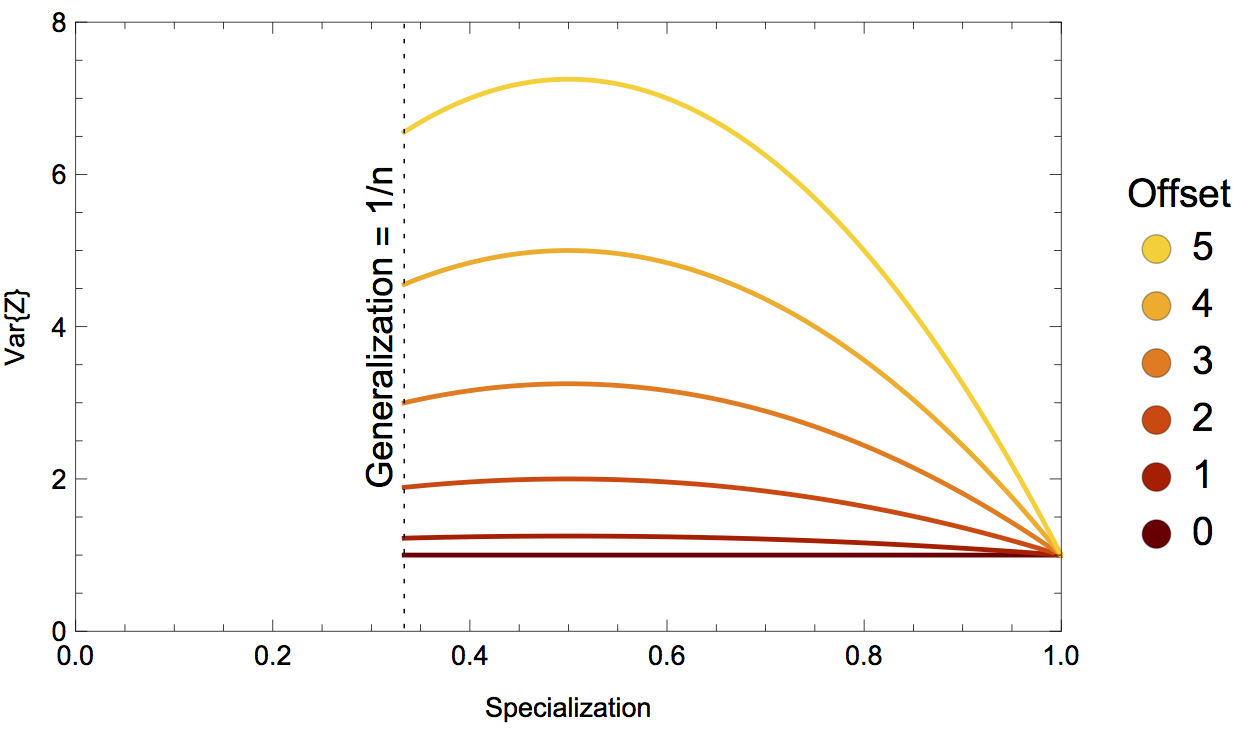
\includegraphics[width=0.5\textwidth]{fig_var.jpg}
\end{center}
\textbf{\refstepcounter{figure}\label{figvar} Figure \arabic{figure}.}{
Variance of the isotopic distribution of a consumer's diet, ${\rm V}\{Z\}$, with respect to specialization on a single prey, $s_k$.
This illustrative example shows a three-prey system with prey means $\{-15,-15+\mbox{offset},-15\}$ and equal variances; colors depect specialization on prey 2 with a mean isotope value that is a function of some offset amount.
As the offset of the targeted prey increases, so does the nonlinearity of ${\rm V}\{Z\}$.
}
\end{figure}

\begin{figure}[h!]
\begin{center}
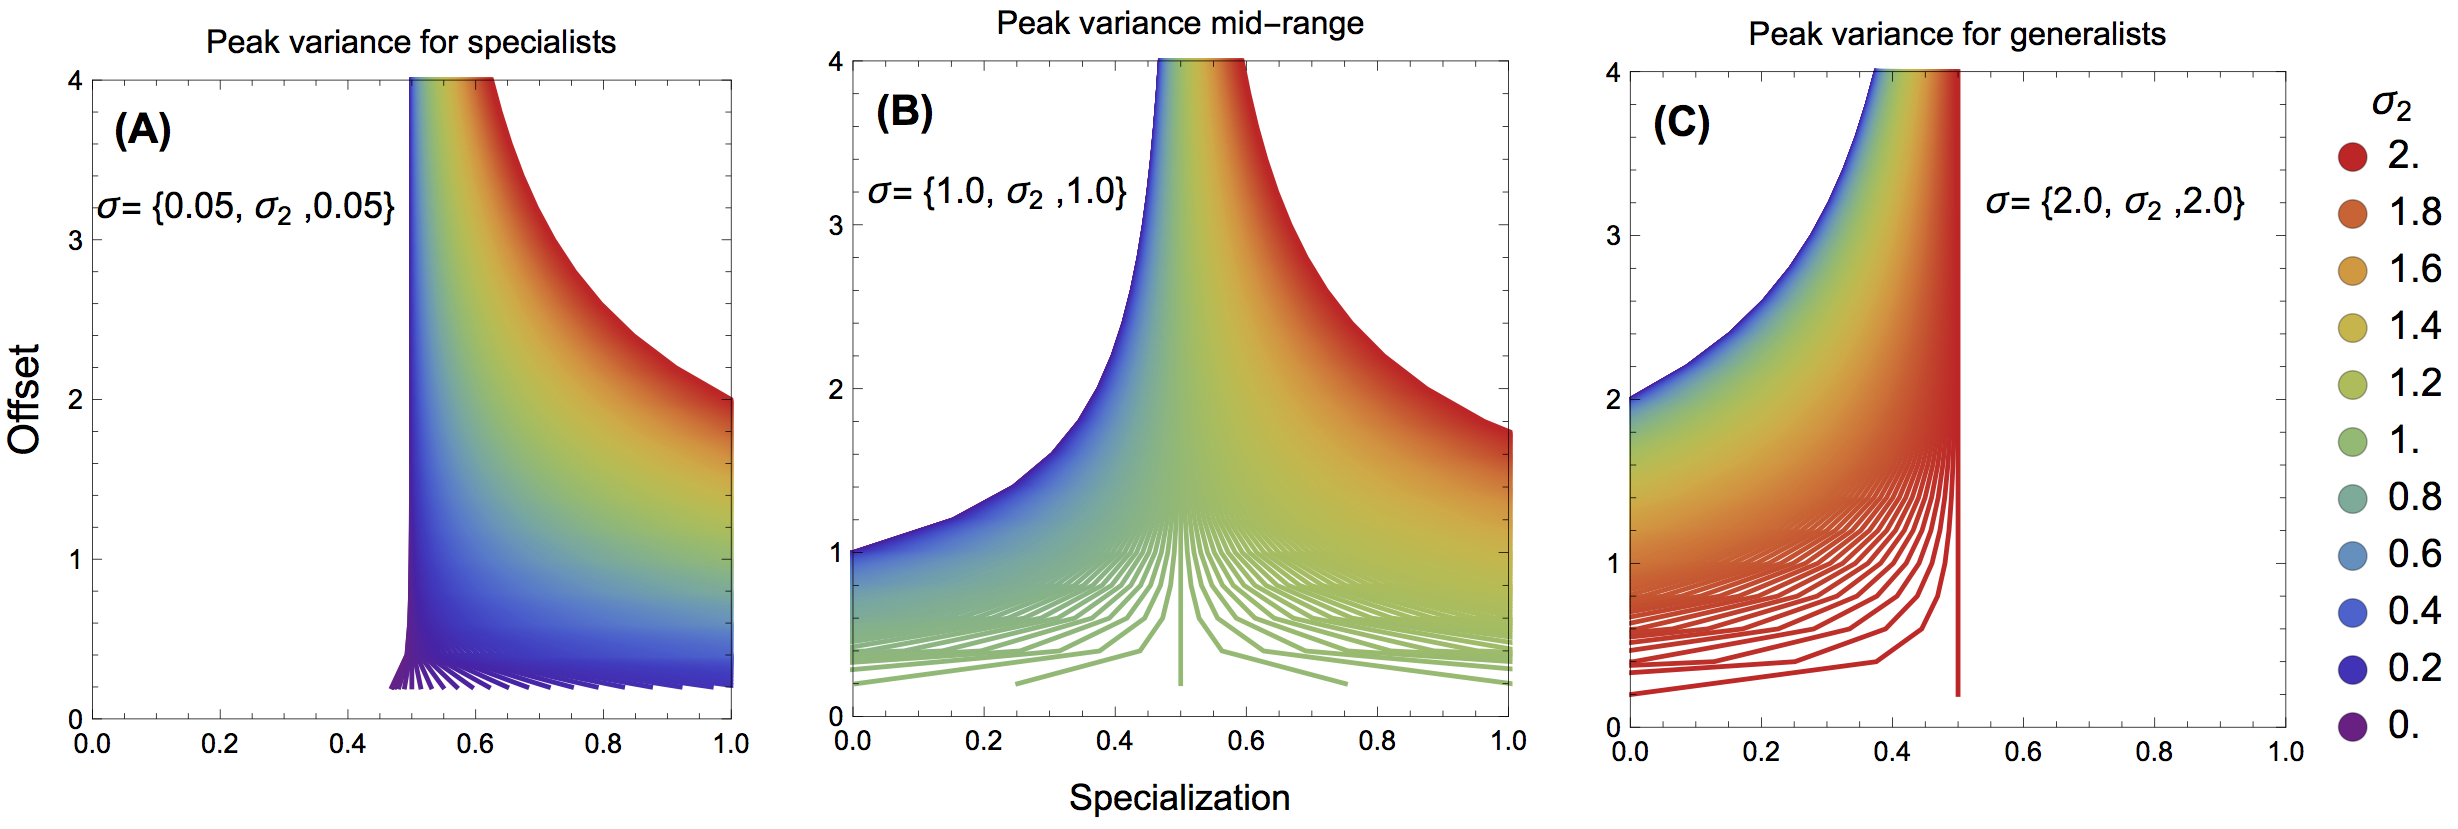
\includegraphics[width=1\textwidth]{fig_specvar.jpg}
\end{center}
\textbf{\refstepcounter{figure}\label{figspecvar} Figure \arabic{figure}.}{
Maximal consumer isotopic variance $\hat s_k$ over the specialization index $s$ as a function of mixing space geometry. 
%A specialization value of $s=1/n$ denotes obligate generalization, while $s=1$ denotes obligate specialization.
%Left, center, and right panel show the effect of different mixing space geometries on the location of maximal consumer niche width over $s$.
{\bf(A)} and {\bf (B)} If the targeted prey has a higher than average isotopic variance, the maximum consumer niche width will lie towards consumer specialization.
{\bf (B)} and {\bf(C)} If the targeted prey has a lower than average isotopic variance, the maximum consumer niche width will like towards consumer generalization.
{\bf(A)}, {\bf (B)}, and {\bf(C)} as the mean offset of the targeted prey is farther from the centroid of the mixing space, the maximal consumer isotopic niche width tends towards $s=0.5$.
}
\end{figure}


\begin{figure}[h!]
\begin{center}
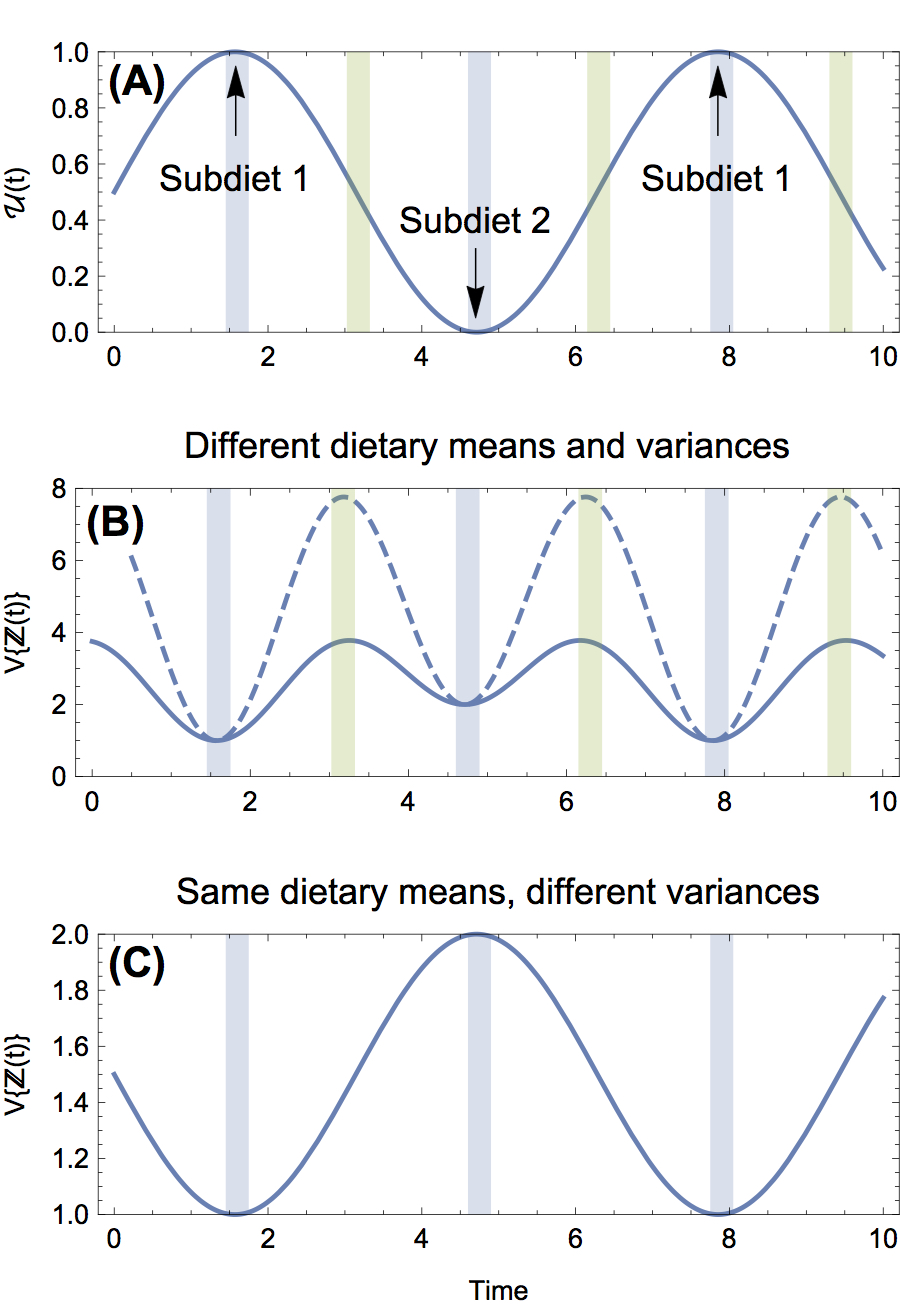
\includegraphics[width=0.4\textwidth]{fig_varZt.jpg}
\end{center}
\textbf{\refstepcounter{figure}\label{figvarZt} Figure \arabic{figure}.}{
{\bf(A)} The proportional contribution of Diet 1 to the composite diet $\mathbb{Z}$ over time.
{\bf(B)} The isotopic variance of the composite diet ${\rm V}\{\mathbb{Z}(t)\}$ when subdiets 1 and 2 have different means and variances. The peak variance occurs during the dietary transitions (green shading), whereas the troughs reflect the variances of subdiet 1 and 2, respectively (blue shading).
{\bf(C)} The isotopic variance of the composite diet ${\rm V}\{\mathbb{Z}(t)\}$ when subdiets 1 and 2 have the same means but different variances. When the subdiets have the same means, ${\rm V}\{\mathbb{Z}(t)\}$ oscillates to reflect the respective variances of the subdiets, and does not exhibit peak variance during the dietary transition.
}
\end{figure}

\begin{figure}[h!]
\begin{center}
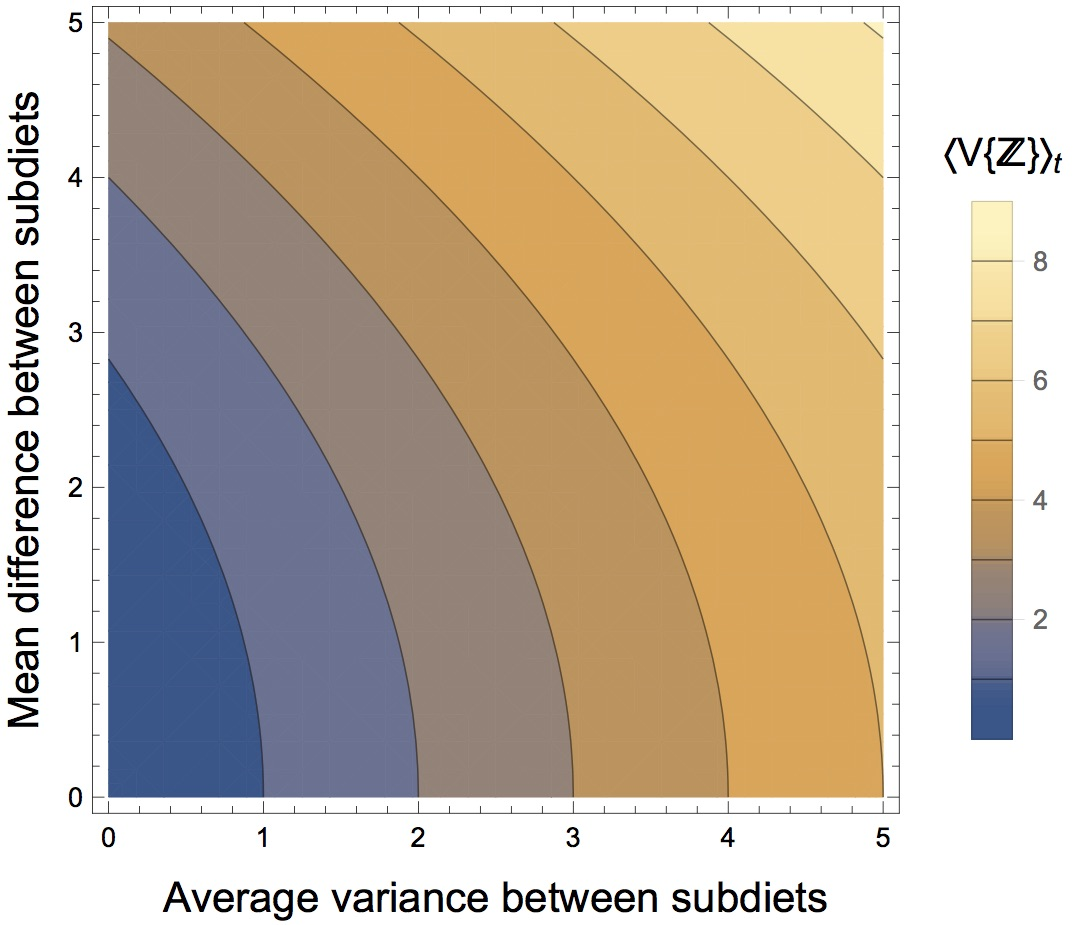
\includegraphics[width=0.4\textwidth]{fig_varzContour.jpg}
\end{center}
\textbf{\refstepcounter{figure}\label{figvarcont} Figure \arabic{figure}.}{
Components of the mixing space that affects the time-averaged variance of the composite diet, $\langle {\rm V}\{\mathbb{Z}\} \rangle_t$.
As the average variance between the subdiets increases, the time-averaged variance of the composite diet increases.
As the difference in the isotopic means of the subdiets increase, the time-averaged variance of the composite diet increases, though at a slower rate.
}
\end{figure}


\begin{figure}[h!]
\begin{center}
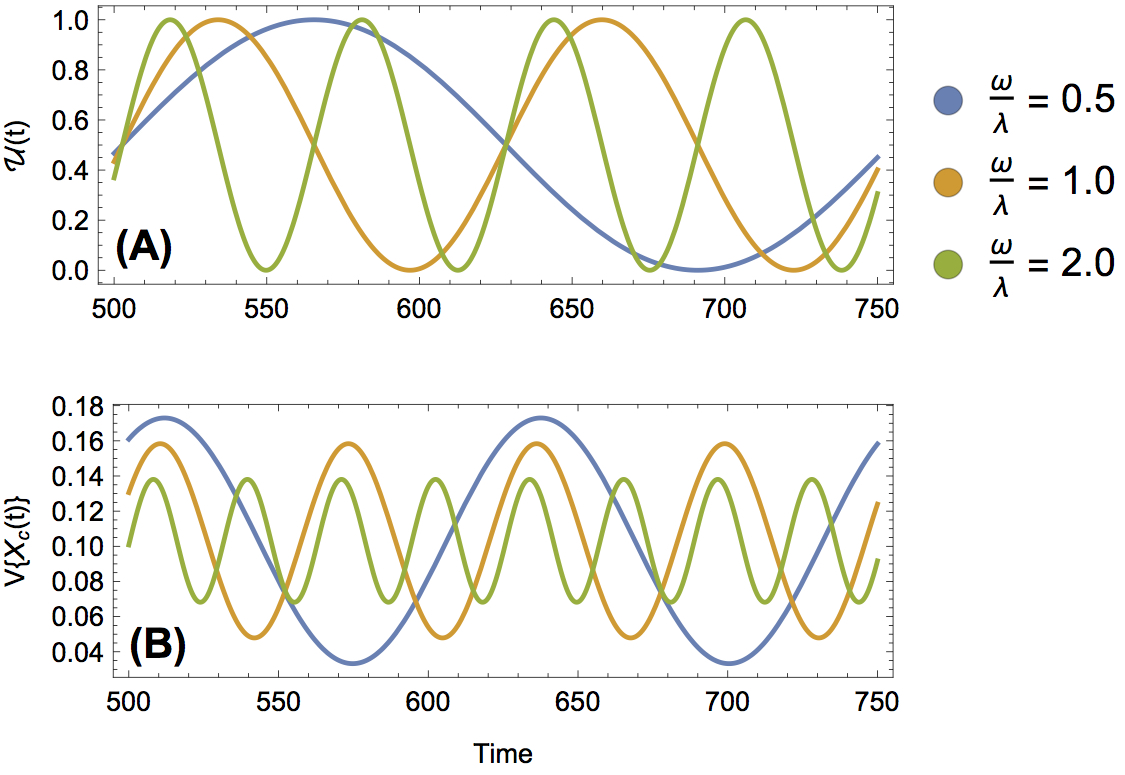
\includegraphics[width=0.5\textwidth]{fig_xcsin.jpg}
\end{center}
\textbf{\refstepcounter{figure}\label{figxcsin} Figure \arabic{figure}.}{
{\bf(A)} A sinusoidally varying diet, where $\mathcal{U}(t) = 1/2 + 1/2\sin(\omega t$) for increasing values of $\omega$, or equivalently, decreasing timescales of dietary switching.
{\bf(B)} The isotopic variance of a consumer over time ${\rm V}\{X_c(t)\}$ across increasing values of $\omega$ relative to the consumer's incorporation rate $\lambda$. 
As the timescale of diet switching decreases relative to the timescale of isotopic incorporation, the amplitude of isotopic variance decreases due to increased isotopic averaging over faster shifts in diet.
}
\end{figure}

\begin{figure}[h!]
\begin{center}
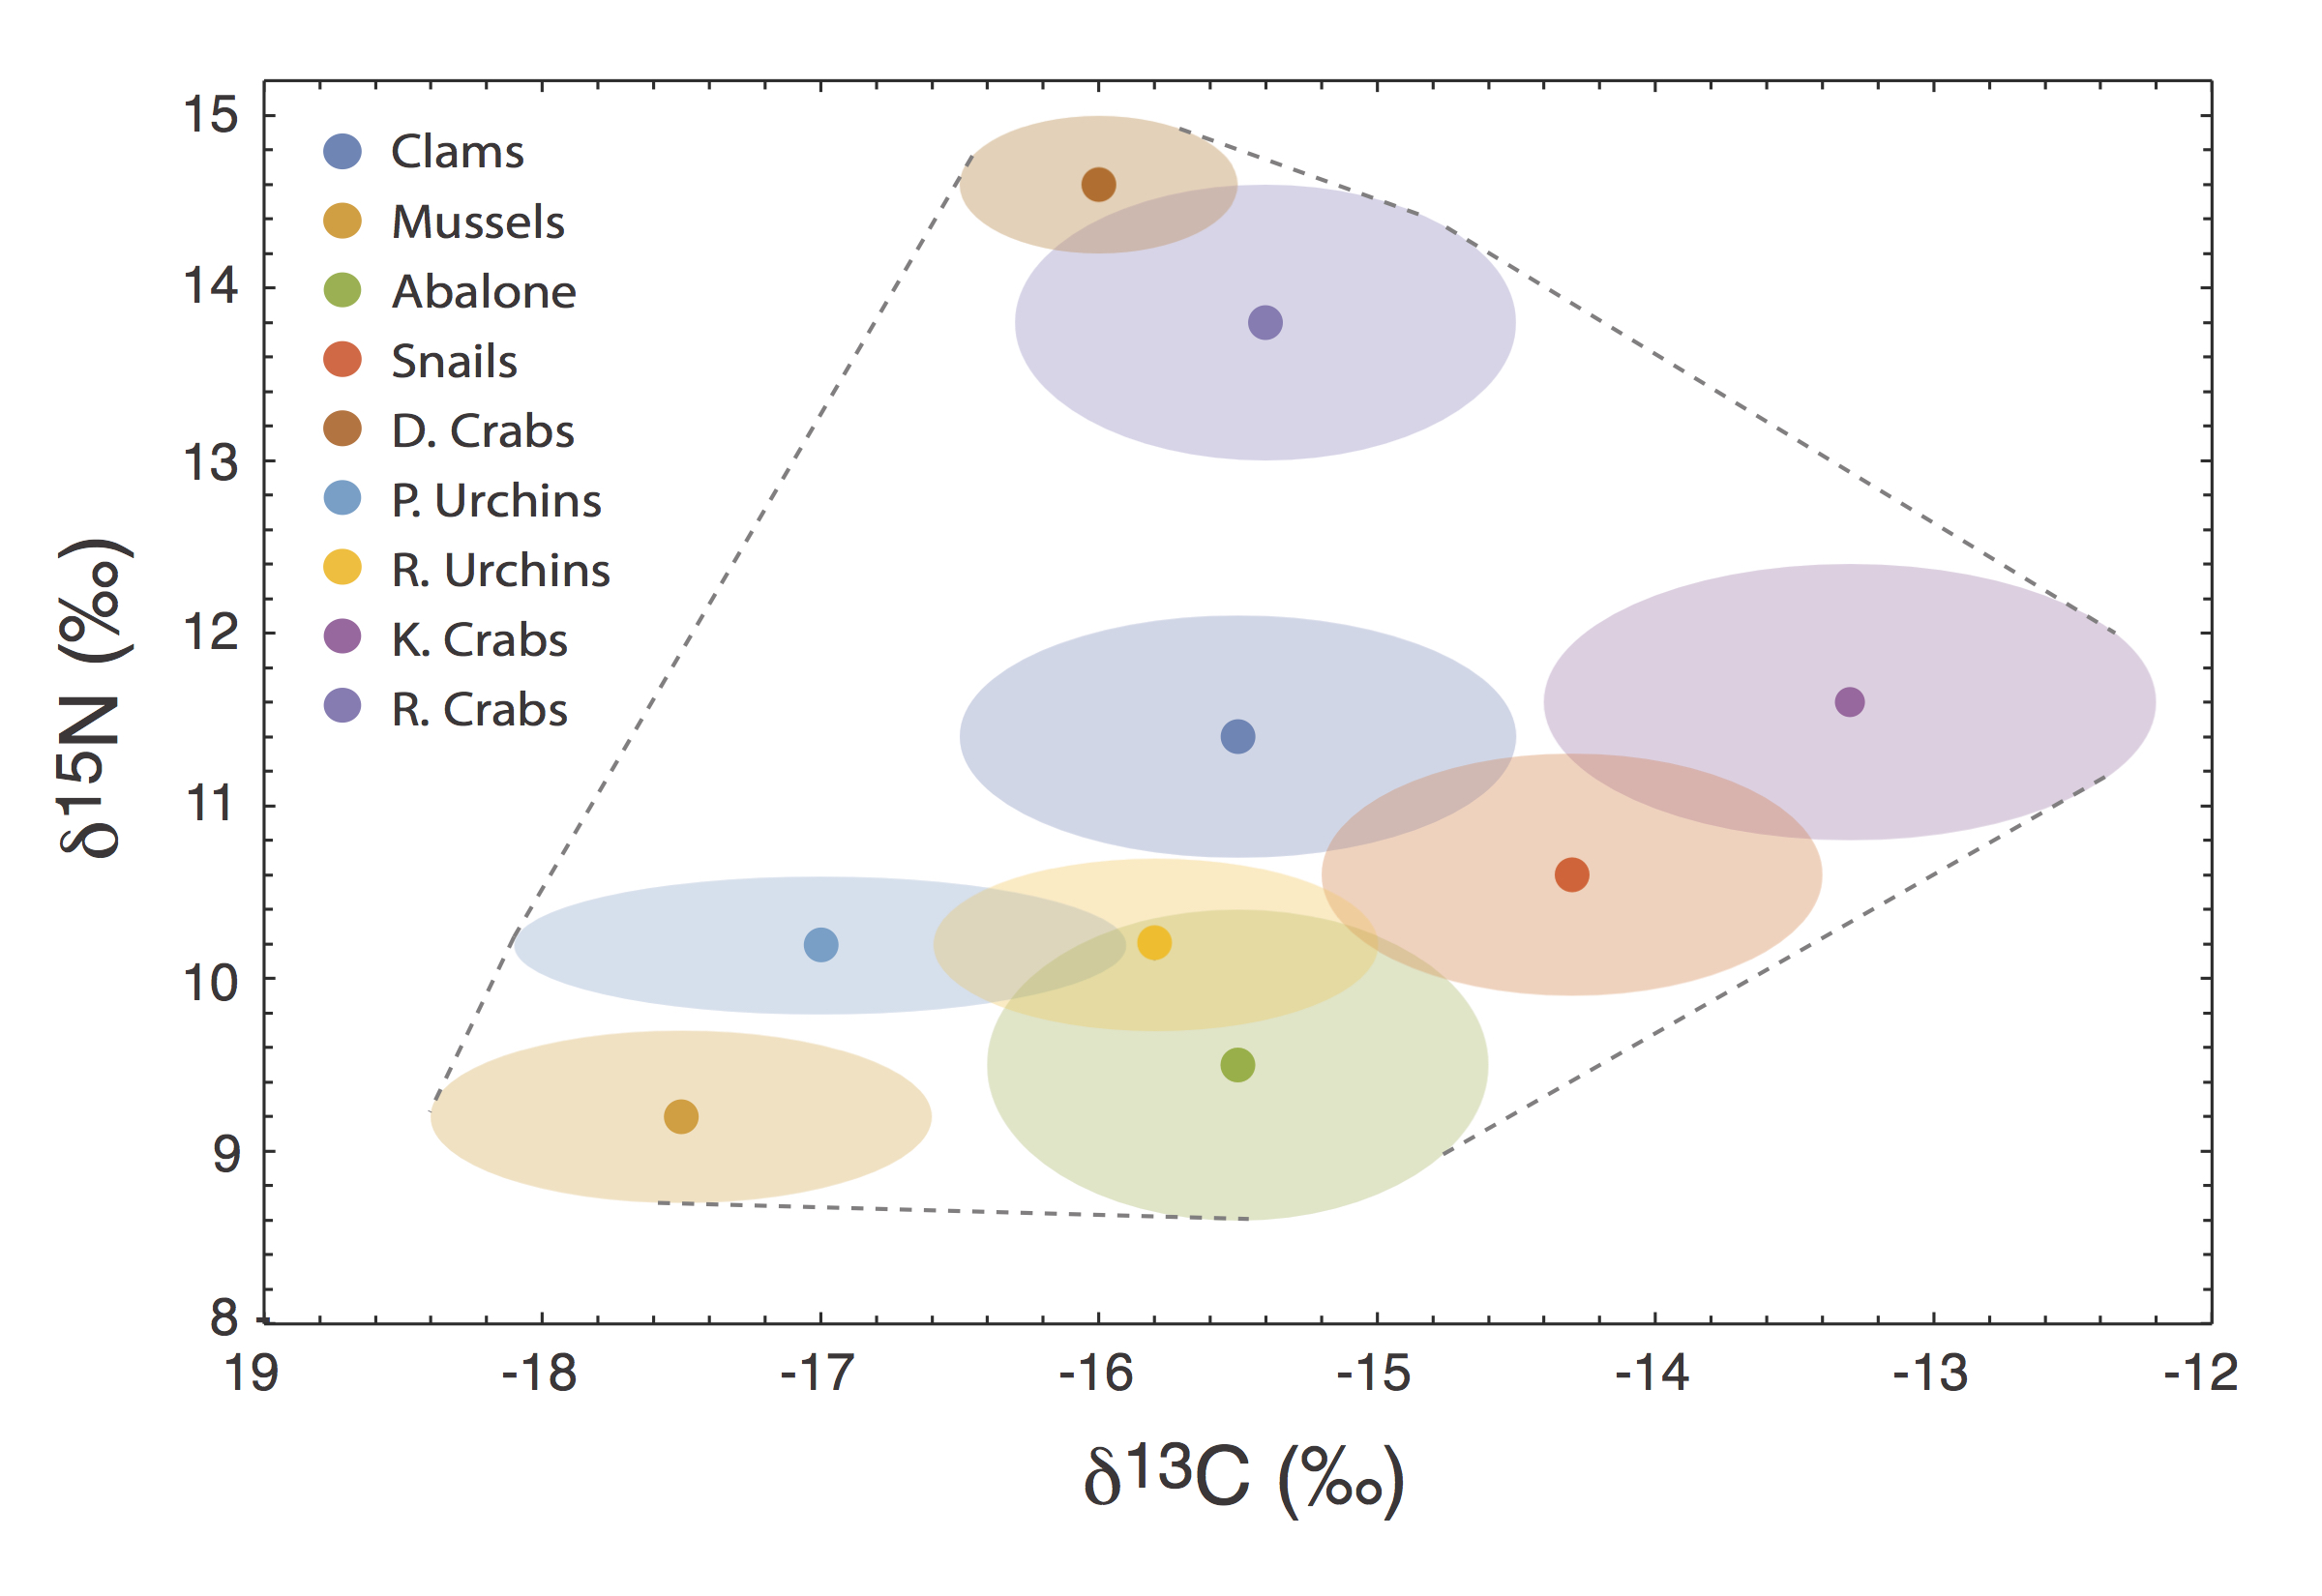
\includegraphics[width=0.65\textwidth]{fig_SOmixing.jpg}
\end{center}
\textbf{\refstepcounter{figure}\label{figsomix} Figure \arabic{figure}.}{
The isotopic mixing space ($\delta^{13}{\rm C}$ vs. $\delta^{15}{\rm N}$) for a sea otter consumer near San Simeon and Monterey Bay, California, composed of nine commonly consumed invertebrate species. Units are per-mil ($\permil$).
}
\end{figure}


\begin{figure}[h!]
\begin{center}
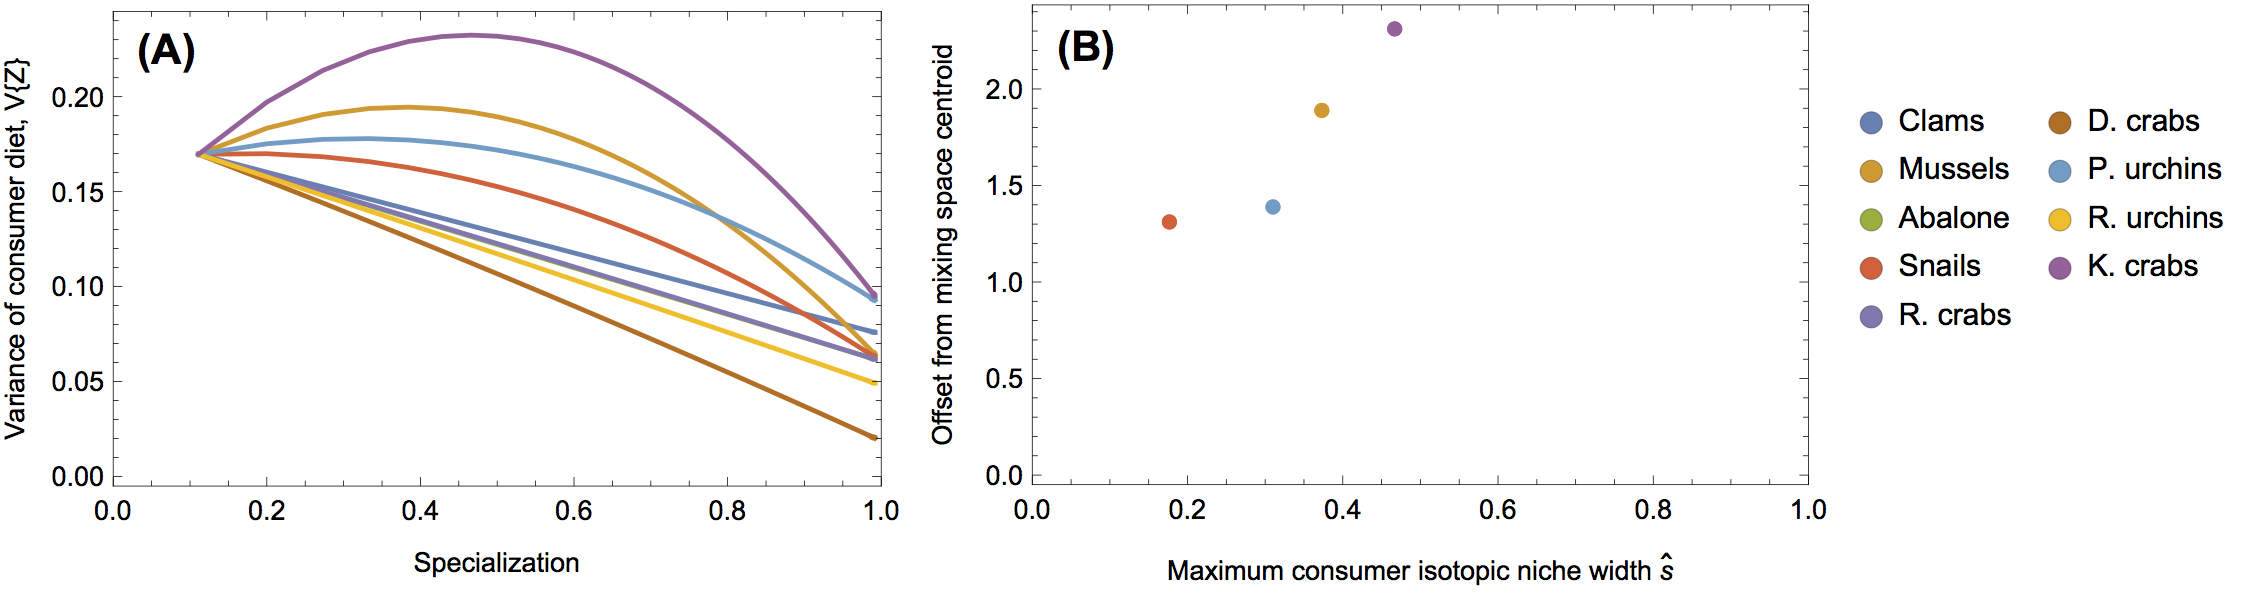
\includegraphics[width=1\textwidth]{fig_ottervar.jpg}
\end{center}
\textbf{\refstepcounter{figure}\label{figottervar} Figure \arabic{figure}.}{
{\bf(A)} Predicted variance in $\delta^{13}{\rm C}$ of sea otter diets over different degrees of specialization on each prey in the system (colors).
{\bf(B)} Calculated maximum consumer niche width values as a function of specialization and the offset of the prey isotopic mean from the mixing space centroid.
}
\end{figure}



\begin{figure}[h!]
\begin{center}
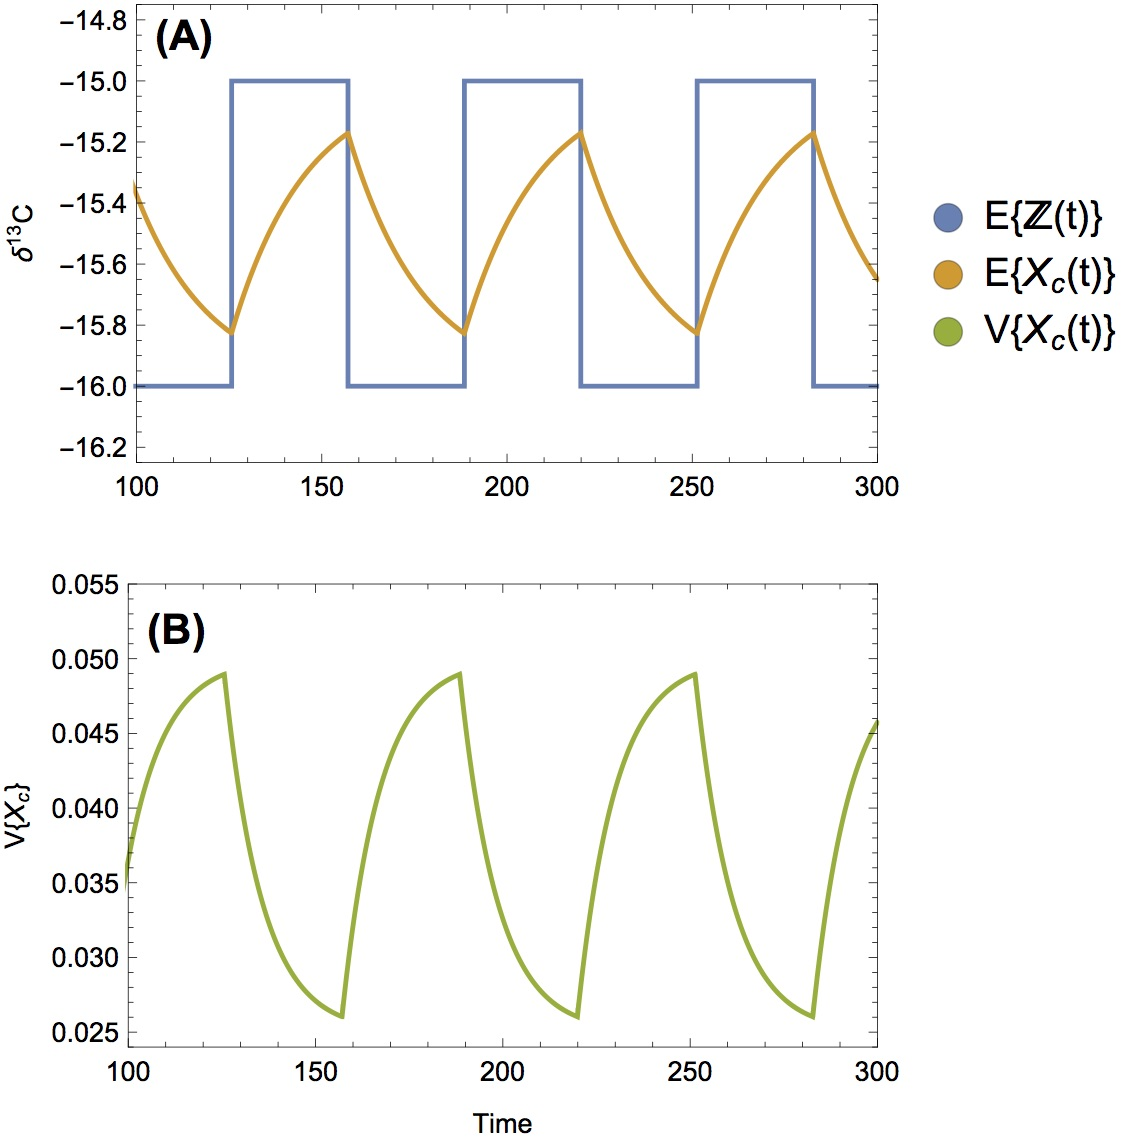
\includegraphics[width=0.5\textwidth]{fig_sawtooth.jpg}
\end{center}
\textbf{\refstepcounter{figure}\label{figsawtooth} Figure \arabic{figure}.}{
{\bf(A)} The mean isotopic value of the composite diet over time ${\rm E}\{\mathbb{Z}(t)\}$ when diet-switching is discontinuous, following a square wave pattern, where subdiets have a mean $\delta^{13}{\rm C}$ value of $-15$ and $-16$, respectively.
The mean isotopic value of the consumer over time ${\rm E}\{X_c(t)\}$ is observed to abruptly change directions when its diet transitions, asymptoting towards (but not reaching) the isotopic mean of its current diet.
{\bf(B)} Consumer isotopic variance ${\rm V}\{X_c(t)\}$ follows a similar trajectory over time, asymptoting towards (but not reaching) the isotope variance of its current diet.
When diets follow a discontinuous switching dynamic, the peak variance does not appear at the transition, as it does when the diet switching is smooth.
}
\end{figure}


\begin{figure}[h!]
\begin{center}
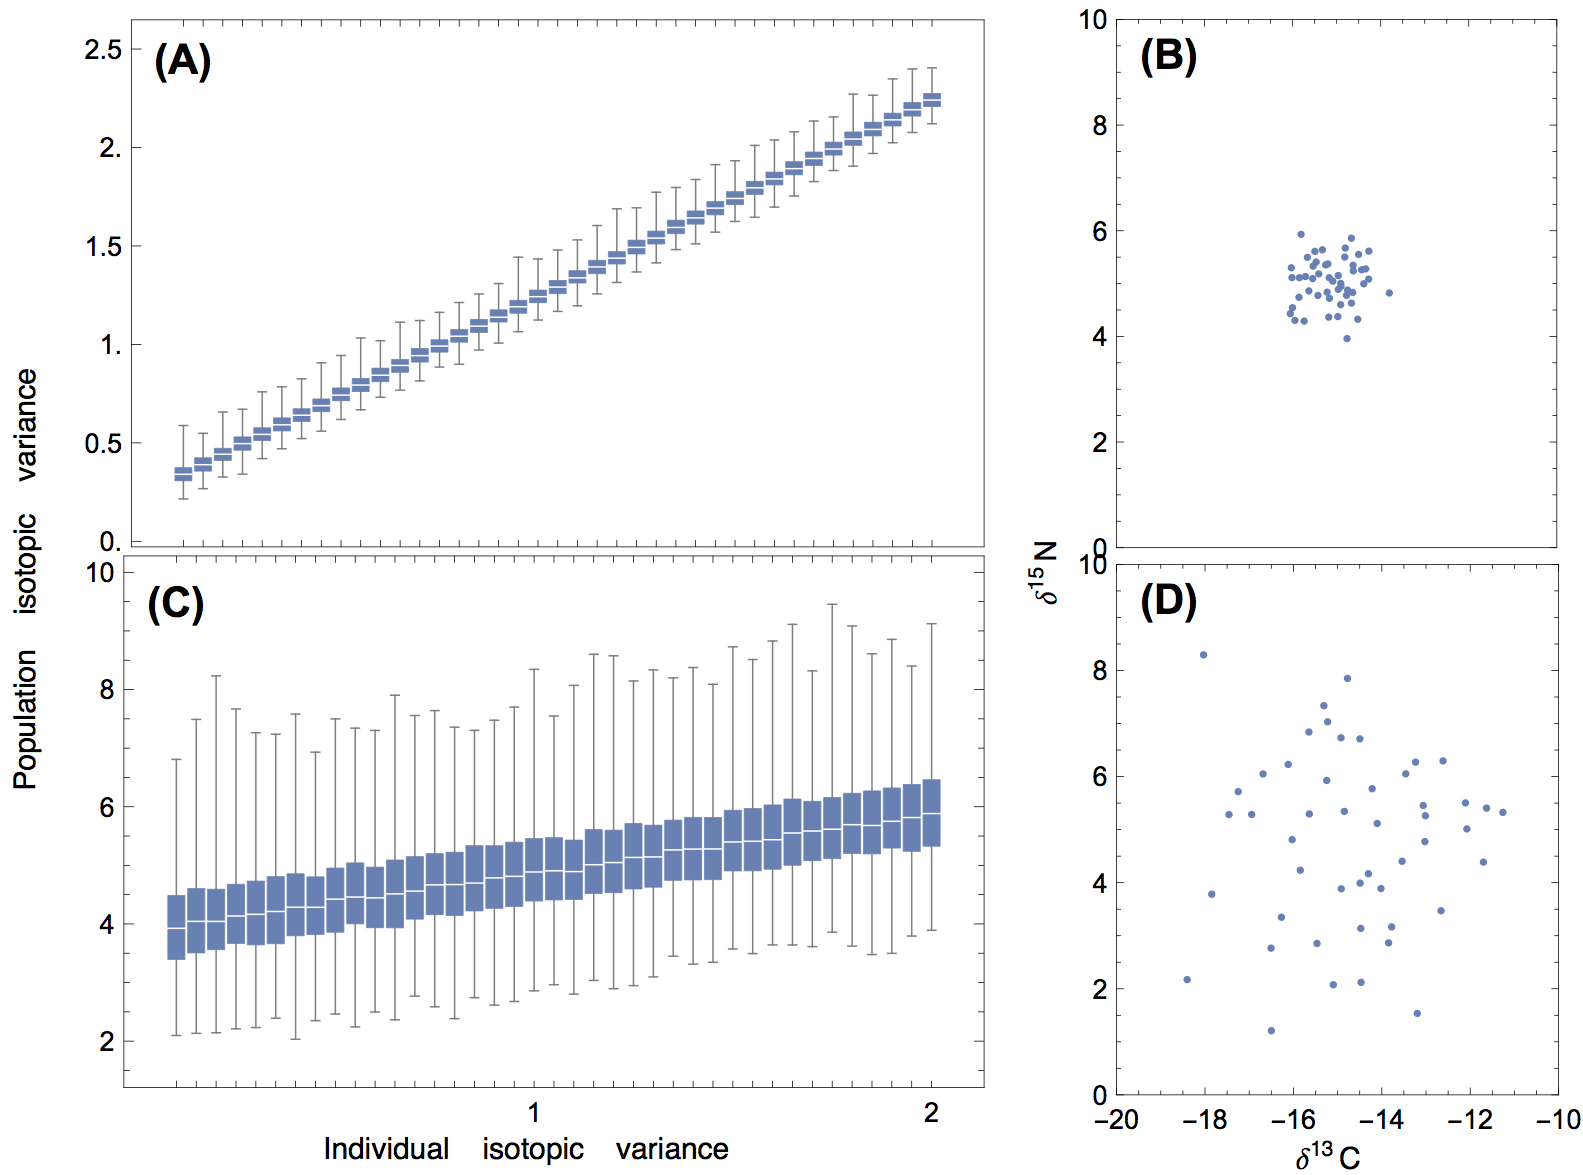
\includegraphics[width=0.75\textwidth]{fig_indpopvar2.jpg}
\end{center}
\textbf{\refstepcounter{figure}\label{figindpopvar} Figure \arabic{figure}.}{
Population isotopic variance vs. individual isotopic variance where mean isotope values of individuals are randomly drawn from a Normal distribution (50 individuals per population; 1000 replicates), and individuals are assumed to have the same variance.
{\bf(A)} and {\bf(B)} When the mean values of individuals are randomly drawn from a normal distribution with low variance, there is a linear relationship between individual-level and population-level isotopic variance.
{\bf(C)} and {\bf(D)} When the mean values of individuals are randomly drawn from a normal distribution with high variance, the relationship becomes masked by noise.
}
\end{figure}



\end{document}
